%~~~~~~~~~~~~~~~~~~~~~~~~~~~~~~~~~~~~~~~~~~~~~~~~~~~~~~~~~~~~~~~~~~~~~~~~~~~~~~~
%
% Diplomarbeitentemplate der |||| HTL Leoben
% zur Verwendung im Fachbereich ITSP
%
% Author: G. Hutter (hg@htl-leoben.at)
%
% Dieses Template generiert alle notwendigen Abschnitte für die Diplomarbeit
% es ist normalerweise nicht notwendig dass die SuS sich mit LaTex herumschlagen
% muessen. 
%
% Vorgehensweise: 
%     - befuellen der Metadaten der Diplomarbeit in der Datei metadata.yaml
%     - markdownfiles mit Inhalt befuellen im ../src/* Ordner
%       Diese werden von pandoc kompiliert und enthalten bereits alle 
%       für die Diplomarbeit notwendigen Abschnittte
%     - Literaturequellen in die Datei literatur.bib
%     - Einzubindende PDFs in das Verzeichnis ./src/pdfs/ einkopieren und
%       dann im yaml File referenzieren
%     - Wenn das Template auf Englisch (oder einer anderen Sprache)
%       verwendet werden soll, dann eiinfach die translations-default.tex auf
%       translations-SPRACHE.tex umkopieren und die Teilstrings ersetzen
%
%~~~~~~~~~~~~~~~~~~~~~~~~~~~~~~~~~~~~~~~~~~~~~~~~~~~~~~~~~~~~~~~~~~~~~~~~~~~~~~~



\documentclass[
    headings=optiontotocandhead,% Erweiterung für das optionale Argument der
                                % Gliederungsbefehle aktiviert.
    twoside,
    numbers=noenddot,% Keine Punkte am Ende der Gliederungsnummern und davon
                     % abgeleiteten Nummern
    %toc=flat, %Flache TOC --- kann man anpassen (auskommentieren)
    12pt, % Schriftgröße 
    titlepage, % es wird eine Titelseite verwendet 
    parskip=full, % Abstand zwischen Absätzen (ganze Zeile) 
    %listof=totoc, % Verzeichnisse im Inhaltsverzeichnis aufführen 
    %listof=flat, % mehr Abstand für grosse Zahlen
    listof=leveldown, 
    numbers=noenddot, % kein Punkt am Ende bei Nummern 
    %%enlargefirstpage,% Gibt es bei scrartcl nicht!!!!
    %bibliography=totoc, % Literaturverzeichnis im Inhaltsverzeichnis aufführen 
    %index=totoc, % Index im Inhaltsverzeichnis aufführen 
    %captions=tableheading, % Beschriftung von Tabellen für Ausgabe oberhalb
                           % der Tabelle formatieren 
    %draft % Status des Dokuments (final/draft) draft hinzufügen zum anziegen 
    %%der zeilen ende
    a4paper,DIV=14,
    BCOR=15mm,
    %captions=tablesignature,
]{scrbook}

%
% verhindert, dass Chapter / Section / Subsection / Subsubsection im Inhaltsverzeichnis so extrem eingerückt werden
%
\makeatletter
\renewcommand*\l@chapter{\bprot@dottedtocline{0}{0em}{2em}}
\renewcommand*\l@section{\bprot@dottedtocline{1}{0em}{3em}}
\renewcommand*\l@subsection{\bprot@dottedtocline{2}{0em}{4em}}
\renewcommand*\l@subsubsection{\bprot@dottedtocline{3}{0em}{5em}}
\makeatother

% Verhindert zu grosse Abstaende beim Inhaltsverzeichnis und gleiche Schriftgoesse wie bei den anderen Ueberschriften
\setkomafont{chapter}{\fontsize{18pt}{18pt}\selectfont}
\BeforeTOCHead[toc]{%
  \KOMAoptions{parskip=false}% no parskip in ToC
  \RedeclareSectionCommand[beforeskip=0mm]{chapter}% no skip after ToC title
}


%
% Farben aus dem HTL Logo
%
\usepackage{color}

\definecolor{htlblau}{RGB}{0,99,169}
\definecolor{htlgrau}{RGB}{153,153,153}
\definecolor{htlgelb}{RGB}{243,172,0}
\definecolor{htlflieder}{RGB}{141,0,76}
\definecolor{htlgruen}{RGB}{63,165,53}


%
% Tabellen und  Bildbezeichnungen
%
\usepackage{booktabs} % Schönere Tabellen machen
\usepackage{caption}
\DeclareCaptionFont{myColor}{\color[RGB]{40,70,119}}
\captionsetup[table]{labelfont=myColor, textfont=myColor}
\captionsetup[longtable]{labelfont=myColor, textfont=myColor}
\captionsetup[figure]{labelfont=myColor, textfont=myColor}
\captionsetup[lstlisting]{labelfont=myColor, textfont=myColor}


%
% this needs to be in the preamble:
\usepackage{chngcntr}
\counterwithout{figure}{chapter}
\counterwithout{figure}{section}

\counterwithout{table}{chapter}
\counterwithout{table}{section}


\setcounter{secnumdepth}{4}
\setcounter{section}{0}

% Schriftart: helvetica
\usepackage[scaled]{helvet}
\renewcommand\familydefault{\sfdefault}

\usepackage[T1]{fontenc}
\usepackage[utf8]{inputenc}


\usepackage{setspace} % Package für 1.5 fachen Zeilenabstand 
\singlespacing        % aber noch nicht jetzt

% Uebersetzungen von Wörtern und Phrasen im Unterordner des Templates
% für neue Sprachen einfach den translations-default.tex Ordner weiterkopieren
% und die Strings neu übersetzen
% Achtung: Der Name sollte so gewählt sein das dazu ein babel Paket existiert
% https://tex.stackexchange.com/questions/330085/how-to-obtain-the-numbered-list-of-languages-loaded-by-babel

\usepackage[english, ngerman ]{babel} % your native language must be the last one!!
\usepackage{translator}
\ProvidesDictionary{translations-default}{default}
\providetranslation{thesis}{Diplomarbeit}
\providetranslation{team}{Team}
\providetranslation{year}{Jahr}
\providetranslation{superisor}{Betreuer}
\providetranslation{missingtitle}{da-titel aus metadata.yaml}
\providetranslation{missingyear}{da-jahr aus metadata.yaml}
\providetranslation{by}{durch}
\providetranslation{executedat}{ausgeführt an der}
\providetranslation{school}{Höheren Technischen Lehranstalt Leoben}
\providetranslation{at}{am}
\providetranslation{signinglocation}{Leoben}
\providetranslation{inyear}{im Schuljahr}
\providetranslation{underSupervisionOf}{unter der Anleitung von}
\providetranslation{signature}{Unterschrift}
\providetranslation{noteofhanks}{Danksagung}
\providetranslation{appendix}{Anhang}
\providetranslation{attachments}{Folgende Dokumente bilden einen Bestandteil dieser Diplomarbeit und liegen der digitalen Version bei.}
\providetranslation{oath}{Ich erkläre hiermit an Eides statt, dass ich die vorliegende Arbeit ohne Hilfe Dritter und ohne Benutzung anderer als der angegebenen Hilfsmittel angefertigt habe; die aus fremden Quellen direkt oder indirekt übernommenen Gedanken sind als solche kenntlich gemacht. Die Arbeit wurde bisher in gleicher oder ähnlicher Form in keiner anderen Prüfungsbehörde vorgelegt und auch noch nicht veröffentlicht. Ich habe keine KI-Tools verwendet, außer in den entsprechend gekennzeichneten Bereichen.}
\providetranslation{of}{der}
\providetranslation{file}{Datei}
\providetranslation{pages}{Seite(n)}
\providetranslation{author}{Autor}
\providetranslation{authorship}{Erklärung der Urheberschaft}
\providetranslation{attachment}{Datei}
\providetranslation{lstoffigures}{Abbildungsverzeichnis}
\providetranslation{lstoftables}{Tabellenverzeichnis}
\providetranslation{lstoflistings}{Quellcodeverzeichnis}
\providetranslation{lstofreferences}{Literaturverzeichnis}


\usedictionary{translations-default}


\usepackage{lastpage}
\usepackage{listings}
\usepackage{blindtext}

%% Aufzählungen nicht so weit einrücken
\usepackage[inline]{enumitem}
%\setitemize{leftmargin=*} 
% Listen etwas wenige einrücken, erfordert enumitem
\setitemize{leftmargin=*}

\usepackage{xspace}
\usepackage{graphicx}

%%? \usepackage{textcomp}
\usepackage[hyphens]{url}
\usepackage{makeidx}
\makeindex
%%? \usepackage{graphicx}
\usepackage[numbers]{natbib}
\PassOptionsToPackage{normalem}{ulem}
\usepackage{ulem}

\usepackage{needspace}

\setlength\partopsep{0.5ex}%schoenere Listen
\usepackage[bottom]{footmisc}%fussnote ganz unten

\usepackage[]{microtype}
\UseMicrotypeSet[protrusion]{basicmath} % disable protrusion for tt fonts

\usepackage{multirow}   % Allows table elements to span several rows.
\usepackage{booktabs}   % Improves the typesettings of tables.
\usepackage{subcaption} % Allows the use of subfigures and enables their referencing.
\usepackage[ruled,linesnumbered,algochapter]{algorithm2e} % Enables the writing of pseudo code.
\usepackage[usenames,dvipsnames,table]{xcolor} % Allows the definition and use of colors. This package has to be included before tikz.
\usepackage{nag}       % Issues warnings when best practices in writing LaTeX documents are violated.
\usepackage{todonotes} % Provides tooltip-like todo notes.
\usepackage{eurosym}   % Euro symbols FTW
\usepackage{censor}    % Zensurierungen (fuer geschwerzte passagen)

% PDF Dateien einbinden lassen (für Appendix)
\usepackage{pdfpages}

\usepackage[binary-units]{siunitx}

%% for pandoc2 images
\makeatletter
\def\maxwidth{\ifdim\Gin@nat@width>\linewidth\linewidth\else\Gin@nat@width\fi}
\def\maxheight{\ifdim\Gin@nat@height>\textheight\textheight\else\Gin@nat@height\fi}
\makeatother
% Scale images if necessary, so that they will not overflow the page
% margins by default, and it is still possible to overwrite the defaults
% using explicit options in \includegraphics[width, height, ...]{}
\setkeys{Gin}{width=\maxwidth,height=\maxheight,keepaspectratio}


%% bessere Suche im PDF
\input{glyphtounicode}
\pdfgentounicode=1


%% Quellcodeformatierung

\usepackage{listings}
\newcommand{\passthrough}[1]{#1}
\lstset{defaultdialect=[5.3]Lua}
\lstset{defaultdialect=[x86masm]Assembler}
\lstset{captionpos=b} % sets the position of the listing headers to bottom

% Redefine the verbatim environment 'Highlighting' to break long lines (with
% the help of fvextra). Redefinition is necessary because it is unlikely that
% pandoc includes fvextra in the default template.
\usepackage{fvextra}
\DefineVerbatimEnvironment{Highlighting}{Verbatim}{breaklines,fontsize=\small,commandchars=\\\{\}}


%
% general listing colors
%
\definecolor{listing-background}{HTML}{F7F7F7}
\definecolor{listing-rule}{HTML}{B3B2B3}
\definecolor{listing-numbers}{HTML}{B3B2B3}
\definecolor{listing-text-color}{HTML}{000000}
\definecolor{listing-keyword}{HTML}{435489}
\definecolor{listing-keyword-2}{HTML}{1284CA} % additional keywords
\definecolor{listing-keyword-3}{HTML}{9137CB} % additional keywords
\definecolor{listing-identifier}{HTML}{435489}
\definecolor{listing-string}{HTML}{00999A}
\definecolor{listing-comment}{HTML}{8E8E8E}

\lstdefinestyle{eisvogel_listing_style}{
  language         = java,
  numbers          = left,
  xleftmargin      = 2.7em,
  framexleftmargin = 2.5em,
  backgroundcolor  = \color{listing-background},
  basicstyle       = \color{listing-text-color}\linespread{1.0}\small\ttfamily{},
  breaklines       = true,
  frame            = single,
  framesep         = 0.19em,
  rulecolor        = \color{listing-rule},
  frameround       = ffff,
  tabsize          = 4,
  numberstyle      = \color{listing-numbers},
  aboveskip        = 1.0em,
  belowskip        = 0.1em,
  abovecaptionskip = 1.0em, % when listing header is on bottom set to 1.0em otherwise 0em
  belowcaptionskip = 0em, % when listing header is on bottom set to 0em otherwise 1.0em
  keywordstyle     = {\color{listing-keyword}\bfseries},
  keywordstyle     = {[2]\color{listing-keyword-2}\bfseries},
  keywordstyle     = {[3]\color{listing-keyword-3}\bfseries\itshape},
  sensitive        = true,
  identifierstyle  = \color{listing-identifier},
  commentstyle     = \color{listing-comment},
  stringstyle      = \color{listing-string},
  showstringspaces = false,
  escapeinside     = {/*@}{@*/}, % Allow LaTeX inside these special comments
  literate         =
  {á}{{\'a}}1 {é}{{\'e}}1 {í}{{\'i}}1 {ó}{{\'o}}1 {ú}{{\'u}}1
  {Á}{{\'A}}1 {É}{{\'E}}1 {Í}{{\'I}}1 {Ó}{{\'O}}1 {Ú}{{\'U}}1
  {à}{{\`a}}1 {è}{{\'e}}1 {ì}{{\`i}}1 {ò}{{\`o}}1 {ù}{{\`u}}1
  {À}{{\`A}}1 {È}{{\'E}}1 {Ì}{{\`I}}1 {Ò}{{\`O}}1 {Ù}{{\`U}}1
  {ä}{{\"a}}1 {ë}{{\"e}}1 {ï}{{\"i}}1 {ö}{{\"o}}1 {ü}{{\"u}}1
  {Ä}{{\"A}}1 {Ë}{{\"E}}1 {Ï}{{\"I}}1 {Ö}{{\"O}}1 {Ü}{{\"U}}1
  {â}{{\^a}}1 {ê}{{\^e}}1 {î}{{\^i}}1 {ô}{{\^o}}1 {û}{{\^u}}1
  {Â}{{\^A}}1 {Ê}{{\^E}}1 {Î}{{\^I}}1 {Ô}{{\^O}}1 {Û}{{\^U}}1
  {œ}{{\oe}}1 {Œ}{{\OE}}1 {æ}{{\ae}}1 {Æ}{{\AE}}1 {ß}{{\ss}}1
  {ç}{{\c c}}1 {Ç}{{\c C}}1 {ø}{{\o}}1 {å}{{\r a}}1 {Å}{{\r A}}1
  {€}{{\EUR}}1 {£}{{\pounds}}1 {«}{{\guillemotleft}}1
  {»}{{\guillemotright}}1 {ñ}{{\~n}}1 {Ñ}{{\~N}}1 {¿}{{?`}}1
  {…}{{\ldots}}1 {≥}{{>=}}1 {≤}{{<=}}1 {„}{{\glqq}}1 {“}{{\grqq}}1
  {”}{{''}}1
}
\lstset{style=eisvogel_listing_style}

% Language definitions are in separate files 
% in order to keep this template somehow readable
% Scala
\lstdefinelanguage{Scala}{
    morekeywords    = {abstract,case,catch,class,def,%
                        do,else,extends,false,final,finally,%
                        for,if,implicit,import,match,mixin,%
                        new,null,object,override,package,%
                        private,protected,requires,return,sealed,%
                        super,this,throw,trait,true,try,%
                        type,val,var,while,with,yield},
    sensitive       = true,
    morecomment     = [l]{//},
    morecomment     = [n]{/*}{*/},
    morestring      = [b]",
    morestring      = [b]',
    morestring      = [b]"""
}

%
% Java (Java SE 12, 2019-06-22)
%
\lstdefinelanguage{Java}{
  morekeywords={
    % normal keywords (without data types)
    abstract,assert,break,case,catch,class,continue,default,
    do,else,enum,exports,extends,final,finally,for,if,implements,
    import,instanceof,interface,module,native,new,package,private,
    protected,public,requires,return,static,strictfp,super,switch,
    synchronized,this,throw,throws,transient,try,volatile,while,
    % var is an identifier
    var
  },
  morekeywords={[2] % data types
    % primitive data types
    boolean,byte,char,double,float,int,long,short,
    % String
    String,
    % primitive wrapper types
    Boolean,Byte,Character,Double,Float,Integer,Long,Short
    % number types
    Number,AtomicInteger,AtomicLong,BigDecimal,BigInteger,DoubleAccumulator,DoubleAdder,LongAccumulator,LongAdder,Short,
    % other
    Object,Void,void
  },
  morekeywords={[3] % literals
    % reserved words for literal values
    null,true,false,
  },
  sensitive,
  morecomment  = [l]//,
  morecomment  = [s]{/*}{*/},
  morecomment  = [s]{/**}{*/},
  morestring   = [b]",
  morestring   = [b]',
}

%JavaScript
\lstdefinelanguage{JavaScript}{
      morekeywords={break, case, catch, continue, debugger, default, delete, 
                    do, else, false, finally, for, function, if, in, instanceof, 
                    new, null, return, switch, this, throw, true, try, typeof, 
                    var, void, while, with},
      morecomment=[s]{/*}{*/},
      morecomment=[l]//,
      morestring=[b]",
      morestring=[b]'
    }

%CSS
\lstdefinelanguage{CSS}{
  keywords={accelerator,azimuth,background,background-attachment,
        background-color,background-image,background-position,
        background-position-x,background-position-y,background-repeat,
        behavior,border,border-bottom,border-bottom-color,
        border-bottom-style,border-bottom-width,border-collapse,
        border-color,border-left,border-left-color,border-left-style,
        border-left-width,border-right,border-right-color,
        border-right-style,border-right-width,border-spacing,
        border-style,border-top,border-top-color,border-top-style,
        border-top-width,border-width,bottom,caption-side,clear,
        clip,color,content,counter-increment,counter-reset,cue,
        cue-after,cue-before,cursor,direction,display,elevation,
        empty-cells,filter,float,font,font-family,font-size,
        font-size-adjust,font-stretch,font-style,font-variant,
        font-weight,height,ime-mode,include-source,
        layer-background-color,layer-background-image,layout-flow,
        layout-grid,layout-grid-char,layout-grid-char-spacing,
        layout-grid-line,layout-grid-mode,layout-grid-type,left,
        letter-spacing,line-break,line-height,list-style,
        list-style-image,list-style-position,list-style-type,margin,
        margin-bottom,margin-left,margin-right,margin-top,
        marker-offset,marks,max-height,max-width,min-height,
        min-width,-moz-binding,-moz-border-radius,
        -moz-border-radius-topleft,-moz-border-radius-topright,
        -moz-border-radius-bottomright,-moz-border-radius-bottomleft,
        -moz-border-top-colors,-moz-border-right-colors,
        -moz-border-bottom-colors,-moz-border-left-colors,-moz-opacity,
        -moz-outline,-moz-outline-color,-moz-outline-style,
        -moz-outline-width,-moz-user-focus,-moz-user-input,
        -moz-user-modify,-moz-user-select,orphans,outline,
        outline-color,outline-style,outline-width,overflow,
        overflow-X,overflow-Y,padding,padding-bottom,padding-left,
        padding-right,padding-top,page,page-break-after,
        page-break-before,page-break-inside,pause,pause-after,
        pause-before,pitch,pitch-range,play-during,position,quotes,
        -replace,richness,right,ruby-align,ruby-overhang,
        ruby-position,-set-link-source,size,speak,speak-header,
        speak-numeral,speak-punctuation,speech-rate,stress,
        scrollbar-arrow-color,scrollbar-base-color,
        scrollbar-dark-shadow-color,scrollbar-face-color,
        scrollbar-highlight-color,scrollbar-shadow-color,
        scrollbar-3d-light-color,scrollbar-track-color,table-layout,
        text-align,text-align-last,text-decoration,text-indent,
        text-justify,text-overflow,text-shadow,text-transform,
        text-autospace,text-kashida-space,text-underline-position,top,
        unicode-bidi,-use-link-source,vertical-align,visibility,
        voice-family,volume,white-space,widows,width,word-break,
        word-spacing,word-wrap,writing-mode,z-index,zoom},  
  sensitive=true,
  morecomment=[l]{//},
  morecomment=[s]{/*}{*/},
  morestring=[b]',
  morestring=[b]",
  alsoletter={:},
  alsodigit={-}
}

%HTML
\lstdefinelanguage{HTML5}{
        language=html,
        sensitive=true, 
        alsoletter={<>=-},
        otherkeywords={
        % HTML tags
        <, </, >,
        </a, <a, </a>,
        </abbr, <abbr, </abbr>,
        </address, <address, </address>,
        </area, <area, </area>,
        </area, <area, </area>,
        </article, <article, </article>,
        </aside, <aside, </aside>,
        </audio, <audio, </audio>,
        </audio, <audio, </audio>,
        </b, <b, </b>,
        </base, <base, </base>,
        </bdi, <bdi, </bdi>,
        </bdo, <bdo, </bdo>,
        </blockquote, <blockquote, </blockquote>,
        </body, <body, </body>,
        </br, <br, </br>,
        </button, <button, </button>,
        </canvas, <canvas, </canvas>,
        </caption, <caption, </caption>,
        </cite, <cite, </cite>,
        </code, <code, </code>,
        </col, <col, </col>,
        </colgroup, <colgroup, </colgroup>,
        </data, <data, </data>,
        </datalist, <datalist, </datalist>,
        </dd, <dd, </dd>,
        </del, <del, </del>,
        </details, <details, </details>,
        </dfn, <dfn, </dfn>,
        </div, <div, </div>,
        </dl, <dl, </dl>,
        </dt, <dt, </dt>,
        </em, <em, </em>,
        </embed, <embed, </embed>,
        </fieldset, <fieldset, </fieldset>,
        </figcaption, <figcaption, </figcaption>,
        </figure, <figure, </figure>,
        </footer, <footer, </footer>,
        </form, <form, </form>,
        </h1, <h1, </h1>,
        </h2, <h2, </h2>,
        </h3, <h3, </h3>,
        </h4, <h4, </h4>,
        </h5, <h5, </h5>,
        </h6, <h6, </h6>,
        </head, <head, </head>,
        </header, <header, </header>,
        </hr, <hr, </hr>,
        </html, <html, </html>,
        </i, <i, </i>,
        </iframe, <iframe, </iframe>,
        </img, <img, </img>,
        </input, <input, </input>,
        </ins, <ins, </ins>,
        </kbd, <kbd, </kbd>,
        </keygen, <keygen, </keygen>,
        </label, <label, </label>,
        </legend, <legend, </legend>,
        </li, <li, </li>,
        </link, <link, </link>,
        </main, <main, </main>,
        </map, <map, </map>,
        </mark, <mark, </mark>,
        </math, <math, </math>,
        </menu, <menu, </menu>,
        </menuitem, <menuitem, </menuitem>,
        </meta, <meta, </meta>,
        </meter, <meter, </meter>,
        </nav, <nav, </nav>,
        </noscript, <noscript, </noscript>,
        </object, <object, </object>,
        </ol, <ol, </ol>,
        </optgroup, <optgroup, </optgroup>,
        </option, <option, </option>,
        </output, <output, </output>,
        </p, <p, </p>,
        </param, <param, </param>,
        </pre, <pre, </pre>,
        </progress, <progress, </progress>,
        </q, <q, </q>,
        </rp, <rp, </rp>,
        </rt, <rt, </rt>,
        </ruby, <ruby, </ruby>,
        </s, <s, </s>,
        </samp, <samp, </samp>,
        </script, <script, </script>,
        </section, <section, </section>,
        </select, <select, </select>,
        </small, <small, </small>,
        </source, <source, </source>,
        </span, <span, </span>,
        </strong, <strong, </strong>,
        </style, <style, </style>,
        </summary, <summary, </summary>,
        </sup, <sup, </sup>,
        </svg, <svg, </svg>,
        </table, <table, </table>,
        </tbody, <tbody, </tbody>,
        </td, <td, </td>,
        </template, <template, </template>,
        </textarea, <textarea, </textarea>,
        </tfoot, <tfoot, </tfoot>,
        </th, <th, </th>,
        </thead, <thead, </thead>,
        </time, <time, </time>,
        </title, <title, </title>,
        </tr, <tr, </tr>,
        </track, <track, </track>,
        </u, <u, </u>,
        </ul, <ul, </ul>,
        </var, <var, </var>,
        </video, <video, </video>,
        </wbr, <wbr, </wbr>,
        />, <!
        },  
        ndkeywords={
        % General
        =,
        % HTML attributes
        accept=, accept-charset=, accesskey=, action=, align=, alt=, async=, autocomplete=, autofocus=, autoplay=, autosave=, bgcolor=, border=, buffered=, challenge=, charset=, checked=, cite=, class=, code=, codebase=, color=, cols=, colspan=, content=, contenteditable=, contextmenu=, controls=, coords=, data=, datetime=, default=, defer=, dir=, dirname=, disabled=, download=, draggable=, dropzone=, enctype=, for=, form=, formaction=, headers=, height=, hidden=, high=, href=, hreflang=, http-equiv=, icon=, id=, ismap=, itemprop=, keytype=, kind=, label=, lang=, language=, list=, loop=, low=, manifest=, max=, maxlength=, media=, method=, min=, multiple=, name=, novalidate=, open=, optimum=, pattern=, ping=, placeholder=, poster=, preload=, pubdate=, radiogroup=, readonly=, rel=, required=, reversed=, rows=, rowspan=, sandbox=, scope=, scoped=, seamless=, selected=, shape=, size=, sizes=, span=, spellcheck=, src=, srcdoc=, srclang=, start=, step=, style=, summary=, tabindex=, target=, title=, type=, usemap=, value=, width=, wrap=,
        % CSS properties
        accelerator:,azimuth:,background:,background-attachment:,
        background-color:,background-image:,background-position:,
        background-position-x:,background-position-y:,background-repeat:,
        behavior:,border:,border-bottom:,border-bottom-color:,
        border-bottom-style:,border-bottom-width:,border-collapse:,
        border-color:,border-left:,border-left-color:,border-left-style:,
        border-left-width:,border-right:,border-right-color:,
        border-right-style:,border-right-width:,border-spacing:,
        border-style:,border-top:,border-top-color:,border-top-style:,
        border-top-width:,border-width:,bottom:,caption-side:,clear:,
        clip:,color:,content:,counter-increment:,counter-reset:,cue:,
        cue-after:,cue-before:,cursor:,direction:,display:,elevation:,
        empty-cells:,filter:,float:,font:,font-family:,font-size:,
        font-size-adjust:,font-stretch:,font-style:,font-variant:,
        font-weight:,height:,ime-mode:,include-source:,
        layer-background-color:,layer-background-image:,layout-flow:,
        layout-grid:,layout-grid-char:,layout-grid-char-spacing:,
        layout-grid-line:,layout-grid-mode:,layout-grid-type:,left:,
        letter-spacing:,line-break:,line-height:,list-style:,
        list-style-image:,list-style-position:,list-style-type:,margin:,
        margin-bottom:,margin-left:,margin-right:,margin-top:,
        marker-offset:,marks:,max-height:,max-width:,min-height:,
        min-width:,transition-duration:,transition-property:,
        transition-timing-function:,transform:,
        -moz-transform:,-moz-binding:,-moz-border-radius:,
        -moz-border-radius-topleft:,-moz-border-radius-topright:,
        -moz-border-radius-bottomright:,-moz-border-radius-bottomleft:,
        -moz-border-top-colors:,-moz-border-right-colors:,
        -moz-border-bottom-colors:,-moz-border-left-colors:,-moz-opacity:,
        -moz-outline:,-moz-outline-color:,-moz-outline-style:,
        -moz-outline-width:,-moz-user-focus:,-moz-user-input:,
        -moz-user-modify:,-moz-user-select:,orphans:,outline:,
        outline-color:,outline-style:,outline-width:,overflow:,
        overflow-X:,overflow-Y:,padding:,padding-bottom:,padding-left:,
        padding-right:,padding-top:,page:,page-break-after:,
        page-break-before:,page-break-inside:,pause:,pause-after:,
        pause-before:,pitch:,pitch-range:,play-during:,position:,quotes:,
        -replace:,richness:,right:,ruby-align:,ruby-overhang:,
        ruby-position:,-set-link-source:,size:,speak:,speak-header:,
        speak-numeral:,speak-punctuation:,speech-rate:,stress:,
        scrollbar-arrow-color:,scrollbar-base-color:,
        scrollbar-dark-shadow-color:,scrollbar-face-color:,
        scrollbar-highlight-color:,scrollbar-shadow-color:,
        scrollbar-3d-light-color:,scrollbar-track-color:,table-layout:,
        text-align:,text-align-last:,text-decoration:,text-indent:,
        text-justify:,text-overflow:,text-shadow:,text-transform:,
        text-autospace:,text-kashida-space:,text-underline-position:,top:,
        unicode-bidi:,-use-link-source:,vertical-align:,visibility:,
        voice-family:,volume:,white-space:,widows:,width:,word-break:,
        word-spacing:,word-wrap:,writing-mode:,z-index:,zoom:
        },  
        morecomment=[s]{<!--}{-->},
        tag=[s]
}



% XML
\lstdefinelanguage{XML}{
  morestring      = [b]",
  moredelim       = [s][\bfseries\color{listing-keyword}]{<}{\ },
  moredelim       = [s][\bfseries\color{listing-keyword}]{</}{>},
  moredelim       = [l][\bfseries\color{listing-keyword}]{/>},
  moredelim       = [l][\bfseries\color{listing-keyword}]{>},
  morecomment     = [s]{<?}{?>},
  morecomment     = [s]{<!--}{-->},
  commentstyle    = \color{listing-comment},
  stringstyle     = \color{listing-string},
  identifierstyle = \color{listing-identifier}
}


% Kotlin
\lstdefinelanguage{Kotlin}{
  comment=[l]{//},
  commentstyle={\color{gray}\ttfamily},
  emph={filter, first, firstOrNull, forEach, lazy, map, mapNotNull, println},
  emphstyle={\color{OrangeRed}},
  identifierstyle=\color{black},
  keywords={!in, !is, abstract, actual, annotation, as, as?, break, by, 
		catch, class, companion, const, constructor, continue, crossinline, 
		data, delegate, do, dynamic, else, enum, expect, external, false, 
		field, file, final, finally, for, fun, get, if, import, in, infix, 
		init, inline, inner, interface, internal, is, lateinit, noinline, 
		null, object, open, operator, out, override, package, param, private, 
		property, protected, public, receiveris, reified, return, return@, 
		sealed, set, setparam, super, suspend, tailrec, this, throw, true, 
		try, typealias, typeof, val, var, vararg, when, where, while},
  keywordstyle={\color{NavyBlue}\bfseries},
  morecomment=[s]{/*}{*/},
  morestring=[b]",
  morestring=[s]{"""*}{*"""},
  ndkeywords={@Deprecated, @JvmField, @JvmName, @JvmOverloads, @JvmStatic, 
		@JvmSynthetic, Array, Byte, Double, Float, Int, Integer, Iterable, 
		Long, Runnable, Short, String, Any, Unit, Nothing},
  ndkeywordstyle={\color{BurntOrange}\bfseries},
  sensitive=true,
  stringstyle={\color{ForestGreen}\ttfamily},
}
%VBA
\lstdefinelanguage{VBA}{
   morekeywords={And, As, Byte, Call, Case, Compare, CDbl, Datebase, Date, 
		Dim, Else, ElseIf, End, Error, Exit, Explicit, False, Function, 
		GoTo, If, IIF, Integer, Not, Nothing, Null, Object, On, Option, Or, 
		Private, Resume, String, Single, Select, Set, Static, Sub, Then, True, To,}, 
   sensitive=false, 
   morecomment=[l]Rem, 
   morecomment=[l]', 
   morestring=[b]", 
   emph={acFormBar, acEditMenu, acCurrent, acEntire, acMenuVer70, acSaveYes, 
		acViewNormal, acForm, acDataErrAdded, acNewRec, acDataErrContinue, Cancel, 
		CancelEvent, Close, CurrentDb, DefaultValue, DateValue, DAO, Description, 
		DoCmd, DoMenuItem, Err, Error, Error$, $, Execute,  FindRecord, Forms, 
		FindFirst, IsNull, Me, MsgBox, GoToControl, GoToRecord, NewData, Nz, 
		Maximize, Number, OpenForm, Parent, Recordset, Requery, Response, SetFocus, 
		stDocName, stLinkCriteria, Value, vbExclamation, vbOK, vbOKCancel, 
		vbInformation, vbYes, vbNo, vbYesNo, vbCancel, vbQuestion, vbYesNoCancel, 
		Visible,}, 
   emphstyle=\itshape} 

\lstdefinelanguage{Dart}{
  morekeywords={
    % normal keywords (without data types)
    abstract, as, assert, async, await, break, case, catch, class, const,
    continue, default, deferred, do, dynamic, else, enum, export, extends,
    extension, external, factory, false, final, finally, for, get, if, implements,
    import, in, interface, is, late, library, mixin, new, null, on, operator,
    part, required, rethrow, return, set, show, static, super, switch, sync,
    this, throw, true, try, typedef, var, void, while, with, yield
  },
  morekeywords={[2] % data types
    int, double, String, bool, List, Map, Set, Future, Stream
  },
  morekeywords={[3] % literals
    % reserved words for literal values
    null,true,false,
  },
  sensitive,
  morecomment  = [l]//,
  morecomment  = [s]{/*}{*/},
  morestring   = [b]",
  morestring   = [b]',
}


%
% Tabellen
%
\usepackage{longtable,booktabs}
% Correct order of tables after \paragraph or \subparagraph
\usepackage{etoolbox}
\makeatletter
\patchcmd\longtable{\par}{\if@noskipsec\mbox{}\fi\par}{}{}
\makeatother
% Allow footnotes in longtable head/foot
\IfFileExists{footnotehyper.sty}{\usepackage{footnotehyper}}{\usepackage{footnote}}
\makesavenoteenv{longtable}

% Gives the opportunity to create a hierarchical directory tree
\usepackage{dirtree} 
% Creates a space before the dirtree
\let\originaldirtree\dirtree
\renewcommand{\dirtree}[1]{
  \vspace{1.5em}
  \originaldirtree{#1}
}

%% Bilder sind oft an merkwürdigen Stellen. Hier regeln wir das indem
%% wir LaTex mitteilen das wir die Bilder GENAU HIER gerne hätten
% Overwrite \begin{figure}[htbp] with \begin{figure}[H]
\usepackage{float}
\let\origfigure=\figure
\let\endorigfigure=\endfigure
\renewenvironment{figure}[1][]{%
   \origfigure[H]
}{%
   \endorigfigure
}

%
% Abbildungsverzeichnis, Tabellenverzeichnis und Quellcodeverzeichnis
% haben eine eigene Überschrift (Section, nicht die selbst mitgbrachte)
%
\makeatletter
\renewcommand{\listoffigures}{\@starttoc{lof}}
\renewcommand{\listoftables}{\@starttoc{lot}}
\renewcommand{\lstlistoflistings}{\@starttoc{lol}}
\makeatother


%
% blockquote
%
\definecolor{blockquote-border}{RGB}{221,221,221}
\definecolor{blockquote-text}{RGB}{119,119,119}
\usepackage{mdframed}
\newmdenv[rightline=false,bottomline=false,topline=false,linewidth=3pt,linecolor=blockquote-border,skipabove=\parskip]{customblockquote}
\renewenvironment{quote}{\begin{customblockquote}\list{}{\rightmargin=0em\leftmargin=0em}%
\item\relax\color{blockquote-text}\ignorespaces}{\unskip\unskip\endlist\end{customblockquote}}

%%%%%%%%%%%%%%%%%%%%%%%%%%%%%%%%%%%%%%%%%%%%%%%%%%%%%%%%%%%%%%%%%%%%%%%%%%%%%%%%%%
%Als erstes „reservieren“ wir den Befehl \authormark mit einer leeren Definition.
\newcommand*{\authormark}{}

%Nun definieren wir \markauthor so, dass er \authormark umdefiniert. Folgende Leerzeichen sollen dabei ignoriert werden.
\newcommand*{\textauthor}[1]{%
   \renewcommand{\authormark}{\translate{author}: #1}%
   \ignorespaces
}

\usepackage[automark,headsepline,footsepline,plainfootsepline]{scrlayer-scrpage}
%\automark[chapter]{chapter}% Eventuell wenn doppelseitig
\setkomafont{pageheadfoot}{\normalcolor\footnotesize\scshape}
\setkomafont{pagenumber}{\normalfont\normalsize}
\clearpairofpagestyles
\ihead{\translate{thesis} 2020/21: \translate{team} Barodscheff, Tester, Ranseier, Borland}
\ohead{\voffset7mm
\includegraphics[width=25mm]{style/HTLLE-Logo.png}}
\ifoot{\authormark}
\ofoot{\pagemark}
\ModifyLayer[addvoffset=-.6ex]{scrheadings.foot.above.line}% Linie verschieben
\ModifyLayer[addvoffset=-.6ex]{plain.scrheadings.foot.above.line}% Linie verschieben
\setlength{\headheight}{32pt}

% alle Seiten mit Kopfzeile
\renewcommand{\chapterpagestyle}{scrheadings}


%% should be last packages
\usepackage{scrhack}


% Sections beginnen immer auf einer neuen Seite
\makeatletter%<-- nur, falls der Code in der Präambel steht
\newcommand*{\the@orig@section}{}
\let\the@orig@section\section
\renewcommand*{\section}{%
  \clearpage
  \the@orig@section
}
\makeatother%<-- nur, falls der Code in der Präambel steht


%% sollte das letzte Package sein
\usepackage[unicode=true,
 bookmarks=true,bookmarksnumbered=false,bookmarksopen=false,
 breaklinks=true,pdfborder={0 0 0},backref=false,colorlinks=false]
 {hyperref}

%
% PDF Metainformationen genereieren und setzen
%
\hypersetup{pdftitle={Erstellen einer Diplomarbeit mit LaTex},
 pdfauthor={Joltawan Barodscheff, Craig Tester, Karl Ranseier, Frank Borland},
 pdfsubject={\translate{Diplomarbeit} HTL Leoben, \translate{year} 2020/21. (\translate{superisor}: hg, me)},
 pdfkeywords={HTLLE, Keyword1, Keyword2, Keyword3}}

\urlstyle{same} % don't use monospace font for urls

%% for pandoc
\providecommand{\tightlist}{%
  \setlength{\itemsep}{0pt}\setlength{\parskip}{0pt}}



% Auch Fußnoten bündig ausrichten
\deffootnote[]{1em}{1em}{\textsuperscript{\thefootnotemark\ }}

%% setup
\sloppy % weniger Meldungen
\voffset7mm % etwas nach unten

%% schöner: 10000 -- gar keine, 1000 als Mittelweg
\clubpenalty = 1000 % Schusterjungen verhindern
\widowpenalty = 1000 % Hurenkinder verhindern
\displaywidowpenalty = 1000 

\renewcommand{\thesection}{\arabic{section}}

%% wir schreiben keine Umlaut mit "a "o
\shorthandoff{"}

%% Paragraphen sind überschriften 4ter Ordnung und sollten auch einen Zeilenumbruch haben.
%% Siehe dazu issue #12
\makeatletter
  \renewcommand\paragraph{\@startsection{paragraph}{4}{\z@}%
    {-3.25ex \@plus -1ex \@minus -0.2ex}%
    {0.01pt}%
    {\raggedsection\normalfont\sectfont\nobreak\size@paragraph}%
  }
\makeatother

%% CSL Referenzen ab pandoc 2.7

%%%%%%%%%%%%%%%%%%%%%%%%%%%%%%%%%%%%%%%%%%%%%%%%%%%%%%%%%%%%%%%%%%%%%%%%%%%%%%%%
\begin{document}


%%%%%%%%%%%%%%%%%%%%%%%%%%%%%%%%%%%%%%%%%%%%%%%%%%%%%%%%%%%%%%%%%%%%%%%%%%%%%%%%
%  DECKBLATT
%%%%%%%%%%%%%%%%%%%%%%%%%%%%%%%%%%%%%%%%%%%%%%%%%%%%%%%%%%%%%%%%%%%%%%%%%%%%%%%%
%\pagenumbering{roman}
\frontmatter % Switches to roman numbering
\title{\translate{thesis}}
\begin{titlepage}

\begin{center}


\includegraphics[width=45mm]{style/HTLLE-Logo.png}

\vspace{2cm}
\textbf{\LARGE{}\translate{thesis}}{\large{}}\\
{\large{}\vspace{15mm}
 \textbf{\large{}
Erstellen einer Diplomarbeit mit LaTex
}\\

 \vspace{15mm}
 \translate{executedat} \\
 \translate{school} \\
 \vspace{1cm}
 \translate{inyear} 
2020/21
\\
 \vspace{1cm}
 \translate{by}\\
 \vspace{0.5cm}
}

\textbf{Barodscheff Joltawan - 5AHWIN} \\ 
Bauen des LaTex Templates
\vspace{5mm}
\\ \textbf{Tester Craig - 5AHWIN} \\ 
Entwicklung eines Prototypen
\vspace{5mm}
\\ \textbf{Ranseier Karl - 5AHWIN} \\ 
API-Mockups und Testen der Applikation
\vspace{5mm}
\\ \textbf{Borland Frank - 5AHWIN} \\ 
GUI Generierung
\vspace{5mm}


\par\end{center}{\large \par}

\begin{center}
 \normalsize \translate{underSupervisionOf} \\
 \vspace{0.5cm}
Ing. DI(FH) Günther Hutter, Msc.\\ DI Dr.~mont Thomas Messner

\par\end{center}

\begin{center}
\vspace{5mm}
\translate{signinglocation}, \today 
\par\end{center}
\end{titlepage}

%%%%%%%%%%%%%%%%%%%%%%%%%%%%%%%%%%%%%%%%%%%%%%%%%%%%%%%%%%%%%%%%%%%%%%%%%%%%%%%%
%  EIDESSTATTLICHE ERKLAERUNGEN
%%%%%%%%%%%%%%%%%%%%%%%%%%%%%%%%%%%%%%%%%%%%%%%%%%%%%%%%%%%%%%%%%%%%%%%%%%%%%%%%
\cleardoublepage{}
\section*{\translate{authorship}}
\translate{oath}

\translate{aitools}

\begin{itemize}[leftmargin=2cm]
\item \textbf{ChatGPT3.5}: Informationsbeschaffung 
\end{itemize}
\begin{itemize}[leftmargin=2cm]
\item \textbf{Midjourney}: Künstlerische Illustration 
\end{itemize}

\noindent

\begin{minipage}[h]{0.4\linewidth}  \vspace*{3cm}
\translate{signinglocation}, \translate{at} \dotfill\\
\vspace*{2.5mm}
\end{minipage}
\hspace*{0.1\linewidth}
\begin{minipage}[h]{0.5\linewidth}  \vspace*{3cm}
  \begin{center}
    \dotfill\\
    (\translate{signature}: Joltawan Barodscheff)
  \end{center}
\end{minipage}
\cleardoublepage{}
\section*{\translate{authorship}}
\translate{oath}

\translate{aitools}

\begin{itemize}[leftmargin=2cm]
\item \textbf{Github Copilot}: Boilerplate codegenerierung, Codedokumentation 
\end{itemize}

\noindent

\begin{minipage}[h]{0.4\linewidth}  \vspace*{3cm}
\translate{signinglocation}, \translate{at} \dotfill\\
\vspace*{2.5mm}
\end{minipage}
\hspace*{0.1\linewidth}
\begin{minipage}[h]{0.5\linewidth}  \vspace*{3cm}
  \begin{center}
    \dotfill\\
    (\translate{signature}: Craig Tester)
  \end{center}
\end{minipage}
\cleardoublepage{}
\section*{\translate{authorship}}
\translate{oath}


\noindent

\begin{minipage}[h]{0.4\linewidth}  \vspace*{3cm}
\translate{signinglocation}, \translate{at} \dotfill\\
\vspace*{2.5mm}
\end{minipage}
\hspace*{0.1\linewidth}
\begin{minipage}[h]{0.5\linewidth}  \vspace*{3cm}
  \begin{center}
    \dotfill\\
    (\translate{signature}: Karl Ranseier)
  \end{center}
\end{minipage}
\cleardoublepage{}
\section*{\translate{authorship}}
\translate{oath}

\translate{aitools}

\begin{itemize}[leftmargin=2cm]
\item \textbf{Galileo AI}: Setendesign sowie UI/UX Design der App 
\end{itemize}
\begin{itemize}[leftmargin=2cm]
\item \textbf{Grammarly Go}: Stilverbesserung sowie Rechtschreibkorrekturen 
\end{itemize}

\noindent

\begin{minipage}[h]{0.4\linewidth}  \vspace*{3cm}
\translate{signinglocation}, \translate{at} \dotfill\\
\vspace*{2.5mm}
\end{minipage}
\hspace*{0.1\linewidth}
\begin{minipage}[h]{0.5\linewidth}  \vspace*{3cm}
  \begin{center}
    \dotfill\\
    (\translate{signature}: Frank Borland)
  \end{center}
\end{minipage}

\onehalfspacing
%%%%%%%%%%%%%%%%%%%%%%%%%%%%%%%%%%%%%%%%%%%%%%%%%%%%%%%%%%%%%%%%%%%%%%%%%%%%%%%%
%  KURZFASSUNG
%%%%%%%%%%%%%%%%%%%%%%%%%%%%%%%%%%%%%%%%%%%%%%%%%%%%%%%%%%%%%%%%%%%%%%%%%%%%%%%%
\cleardoublepage{}
\section*{Kurzfassung}
Hier kommt eine deutsche Kurzfassung hin.

%%%%%%%%%%%%%%%%%%%%%%%%%%%%%%%%%%%%%%%%%%%%%%%%%%%%%%%%%%%%%%%%%%%%%%%%%%%%%%%%
%  ABSTRACT
%%%%%%%%%%%%%%%%%%%%%%%%%%%%%%%%%%%%%%%%%%%%%%%%%%%%%%%%%%%%%%%%%%%%%%%%%%%%%%%%
\cleardoublepage{}
\section*{Abstract}
Hier kommt eine englische Kurzfassung hin.

%%%%%%%%%%%%%%%%%%%%%%%%%%%%%%%%%%%%%%%%%%%%%%%%%%%%%%%%%%%%%%%%%%%%%%%%%%%%%%%%
%  DANKSAGUNG
%%%%%%%%%%%%%%%%%%%%%%%%%%%%%%%%%%%%%%%%%%%%%%%%%%%%%%%%%%%%%%%%%%%%%%%%%%%%%%%%


%%%%%%%%%%%%%%%%%%%%%%%%%%%%%%%%%%%%%%%%%%%%%%%%%%%%%%%%%%%%%%%%%%%%%%%%%%%%%%%%
%  INHALTSVERZEICHNIS
%%%%%%%%%%%%%%%%%%%%%%%%%%%%%%%%%%%%%%%%%%%%%%%%%%%%%%%%%%%%%%%%%%%%%%%%%%%%%%%%
\cleardoublepage{}
\setcounter{tocdepth}{3}
\tableofcontents{}

%%%%%%%%%%%%%%%%%%%%%%%%%%%%%%%%%%%%%%%%%%%%%%%%%%%%%%%%%%%%%%%%%%%%%%%%%%%%%%%%
%  Markdown generierter content
%%%%%%%%%%%%%%%%%%%%%%%%%%%%%%%%%%%%%%%%%%%%%%%%%%%%%%%%%%%%%%%%%%%%%%%%%%%%%%%%
%hier geht es los mit dem Text - auf einer rechten Seite
\raggedbottom
\cleardoublepage{}
\mainmatter
\hypertarget{einleitung}{%
\section{Einleitung}\label{einleitung}}

Hier schreiben Sie eine Einleitung zu Ihrem Thema Das ist quasi der
Problemaufriss

\hypertarget{zielsetzung}{%
\section{Zielsetzung}\label{zielsetzung}}

Die Zielsetzung beschreibt das allgemeine Ziel der Diplomarbeit. Dabei
sollten folgende Themen behandelt werden:

\begin{itemize}
\tightlist
\item
  Was ist der aktuelle Stand in der Firma / am Projekt an dem Sie
  arbeiten?
\item
  Was ist die Motiavation hinter dieser Arbeit?
\item
  Was möchten Sie erreichen ?
\item
  Was möchten Sie nicht erreichen ? (Nicht-Ziele)
\item
  Was ändert sich wenn Sie diese Arbeit schreiben ?
\end{itemize}

Die konkreten Ausarbeitungen sind in den n- Unterfiles (je Schüler
eines) abzubilden.

\hypertarget{aufgabenstellung}{%
\section{Aufgabenstellung}\label{aufgabenstellung}}

\hypertarget{auftraggeber}{%
\subsection{Auftraggeber}\label{auftraggeber}}

Wer ist der Auftraggeber, wie ist es zu dieser Arbeit gekommen, was
verspricht sich der Auftraggeber davon

\hypertarget{ausgangssituation}{%
\subsection{Ausgangssituation}\label{ausgangssituation}}

Eine allgemeine Aufgabenstellung

\begin{itemize}
\tightlist
\item
  Was ist die derzeitige Situation ?
\item
  Wie wird derzeit gearbeitet ?
\end{itemize}

\hypertarget{so-gehen-zitate}{%
\subsubsection{So gehen Zitate}\label{so-gehen-zitate}}

Hier ein einzel Zitat eines Buches das auf der Seite 17 zu finden ist:\\
({[}\protect\hyperlink{ref-hattie_lernen_2013}{1}{]} S. 17)

Zitatsammlung:\\
(vergleich dazu \protect\hyperlink{ref-heise}{2} oder
\protect\hyperlink{ref-t3n}{3})\\
{[}\protect\hyperlink{ref-hattie_lernen_2013}{1},\protect\hyperlink{ref-leeb_einfuhrung_2016}{4}{]}

Zitat ohne Autor\\
Hattie sagte bla bla {[}\protect\hyperlink{ref-hattie_lernen_2013}{1}{]}

Name des Autors mit Jahr in Klammern\\
\protect\hyperlink{ref-hattie_lernen_2013}{1} sagte einmal bla bla bla

Auch Videos kann man Zitieren wi Zum Biespiel hier
{[}\protect\hyperlink{ref-Zatko15}{5}{]} in dieser Referenz.

Hier noch ein Zitat mit Seitenangabe
{[}{[}\protect\hyperlink{ref-Zatko15}{5}{]} Seite 5f.{]}

Man darf auch ChatGPT oder andere KIs befragen um Wissen zu erlangen.
Dazu muss allerdings ein PDF Log des exakten Chats in die Metadata.yaml
eingetragen werden und der dort eingetragene
\passthrough{\lstinline!short-prompt!} auch in der bib Datei eingefügt
werden. Dann könnten indirekte Zitate so aussehen
{[}\protect\hyperlink{ref-gpt-pandoc}{6}{]} oder auch so
{[}\protect\hyperlink{ref-gpt-atomaufbau}{7}{]}.

Wichtig ist es, das beim Author die verwendete KI eingetragen wird (mit
Versionsnummern - so genau wie möglich), beim title eine kurze Referenz
zum Prompt und beim Jahr - das Jahr in dem die Abfrage gemacht wurde.
Das hat dem \passthrough{\lstinline!short-prompt!} aus der metadata.yaml
zu entsprechen.

\begin{lstlisting}
@unpublished{gpt-pandoc,
  author = {{ChatGPT 4.0}},
  title  = {Was ist Pandoc ?},
  year   = {2024},
  url={https://chat.openai.com/c/ef535195-0e39-4d5c-9c85-cdb7ec18ad03},
  urldate = {2023-02-29}
}
\end{lstlisting}

Oben sieht man wie ein korrekter Bibtech Eintrag für eine ChatGPT
Konversation aussieht. Zusätzlich wurden hier bei URL noch die url des
Chats eingetragen - was zwar praktisch ist, uns allerdings nicht von der
Pflicht entbindet den Chatverlauf in der DA als PDF einzufügen.
Anzumerkein ist ebenfalls noch das wir hier ein
\passthrough{\lstinline!unpublished!} Tag verwenden weil wir hier eben
Quellen verwenden die in dieser Form nicht gepublished wurden.

\hypertarget{systembeschreibung-y}{%
\subsubsection{Systembeschreibung Y}\label{systembeschreibung-y}}

\hypertarget{systembeschreibung-z}{%
\subsubsection{Systembeschreibung Z}\label{systembeschreibung-z}}

\hypertarget{teilaufgabe-schuxfcler-barodscheff}{%
\section{Teilaufgabe Schüler
Barodscheff}\label{teilaufgabe-schuxfcler-barodscheff}}

\textauthor{Joltawan Barodscheff}

Dieses Kapitel wird oft auch als \emph{Literaturrecherche} bezeichnet.
Da gehört alles rein was der \textbf{normale} Leser braucht um den
praktischen Ansatz zu verstehen. Das bedeutet Sie brauchen einen roten
Faden !

Das sind z.B: allgemeine Definitionen, Beschreibung von fachspezifischen
Vorgehensweisen, Frameworks, Theorie zu verwendeten Algorithmen,
besondere Umstände, \ldots{}

\hypertarget{praktische-arbeit}{%
\subsection{Praktische Arbeit}\label{praktische-arbeit}}

\begin{quote}
Hier beschreiben Sie ihren praktischen Teil. Es geht darum seine
Implementierung / Versuche so darzustellen dass anhand dieser dre Leser
erkennen kann was sie wie gemacht haben.
\end{quote}

Die Frage nach der Detailgenauigkeit lässt sich wie folgt beantworten:
So, dass man Ihre Aufgabenstellung vollständig nachvollziehen kann wenn
man nur diese Diplomarbeit in Händen hat!

\hypertarget{messergebnisse}{%
\subsubsection{Messergebnisse}\label{messergebnisse}}

\begin{figure}
\centering
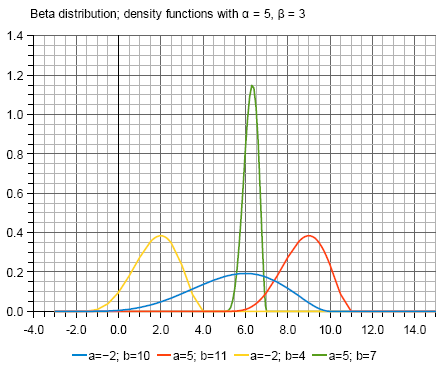
\includegraphics[width=0.7\textwidth,height=\textheight]{img/graph.png}
\caption{Ein PNG Bild\label{fig:png_bild}}
\end{figure}

Bilder sind so scharf wie möglich darzustellen. Unnötige Dinge (welche
für den Leser keine Information liefern) sind wegzuschneiden.
Üblicherweise versucht das Framework Bilder möglichst gut und
vollflächig in die Seite einzupassen - was aber speziell bei kleinen
Bildern keinen Sinn macht. Daher kann man die Breite des Bildes
\passthrough{\lstinline!\{width=xx\%\}!} beeinflussen. Generell macht es
keinen Sinn reisen Bilder mit dieser Funktion niederzuskalieren, sondern
eher die Bilder schon vorher mittels eines Bildbearbeitungsprogrammes
niederzurechnen. Damit wird das endgültige PDF nicht so groß.

\hypertarget{etwas-fliesstext}{%
\subsubsection{Etwas Fliesstext}\label{etwas-fliesstext}}

We'll put some happy little leaves here and there. Poor old tree. Have
fun with it. Isn't that fantastic? You can just push a little tree out
of your brush like that.

Making all those little fluffies that live in the clouds. If there's two
big trees invariably sooner or later there's gonna be a little tree.
There is no right or wrong - as long as it makes you happy and doesn't
hurt anyone. Use absolutely no pressure. Just like an angel's wing. This
is the time to get out all your flustrations, much better than kicking
the dog around the house or taking it out on your spouse. I guess I'm a
little weird. I like to talk to trees and animals. That's okay though; I
have more fun than most people.

\todo{Noch weitere Infos einholen}

Do an almighty painting with us. Learn when to stop. Absolutely no
pressure. You are just a whisper floating across a mountain. As trees
get older they lose their chlorophyll. Clouds are free. They just float
around the sky all day and have fun.

Now a hierarchical tree from this repo:

\dirtree{%
.1 ./.
.2 example.
.3 ....
.2 style.
.3 ....
.2 tools.
.3 docker.
.3 github.
.2 Jenkinsfile.
.2 Makefile.
.2 REAMDE.md.
}

A fan brush can be your best friend. Sometimes you learn more from your
mistakes than you do from your masterpieces. You can bend rivers. But
when I get home, the only thing I have power over is the garbage. Don't
kill all your dark areas - you need them to show the light. There's
nothing wrong with having a tree as a friend.

God gave you this gift of imagination. Use it. Use your imagination, let
it go. Put your feelings into it, your heart, it's your world. There's
not a thing in the world wrong with washing your brush. Happy painting,
God bless. All those little son of a guns.

I sincerely wish for you every possible joy life could bring. Everybody
needs a friend. That's crazy.

If you don't like it - change it. It's your world. Isn't it great to do
something you can't fail at? Play with the angles. See how easy it is to
create a little tree right in your world. This piece of canvas is your
world. This painting comes right out of your heart.

\hypertarget{teilaufgabe-schuxfcler-bravo}{%
\section{Teilaufgabe Schüler Bravo}\label{teilaufgabe-schuxfcler-bravo}}

\textauthor{Schueler 2}

\hypertarget{theorie}{%
\subsection{Theorie}\label{theorie}}

Dieses Kapitel wird oft auch als \emph{Literaturrecherche} bezeichnet.
Da gehört alles rein was der \textbf{normale} Leser braucht um den
praktischen Ansatz zu verstehen. Das bedeutet Sie brauchen einen roten
Faden !

Das sind z.B: allgemeine Definitionen, Beschreibung von fachspezifischen
Vorgehensweisen, Frameworks, Theorie zu verwendeten Algorithmen,
besondere Umstände, \ldots{}

\hypertarget{praktische-arbeit-1}{%
\subsection{Praktische Arbeit}\label{praktische-arbeit-1}}

Hier beschreiben Sie ihren praktischen Teil. Es geht darum seine
Implementierung / Versuche so darzustellen dass anhand dieser dre Leser
erkennen kann was sie wie gemacht haben.

Die Frage nach der Detailgenauigkeit lässt sich wie folgt beantworten:
So, dass man Ihre Aufgabenstellung vollständig nachvollziehen kann wenn
man nur diese Diplomarbeit in Händen hat!

\hypertarget{erzeugen-von-java-quellcode}{%
\subsubsection{Erzeugen von Java
Quellcode}\label{erzeugen-von-java-quellcode}}

Unter einem Array in Java versteht man ein Feld oder Container, das in
der Lage ist, mehrere Objekte vom gleichen Typ aufzunehmen und zu
verwalten. Dabei wird in Java das Array als eine spezielle Klasse
repräsentiert, was unter anderem mit sich bringt, dass man auf spezielle
Methoden und Operationen bei Arrays zurückgreifen kann. Der Umgang mit
Arrays mag gerade am Anfang etwas schwerer sein und birgt viele
Fehlerquellen, nach und nach wird man das System das hinter den Arrays
steht aber gut nachvollziehen können.

\begin{lstlisting}[language=Java, caption={Initialisieren eines Arrays}]
Typ[] Name = new Typ[Anzahl];
Typ Name[] = new Typ[Anzahl];
\end{lstlisting}

Etwas erfahrenere Programmierer werden jetzt schon erkennen, worauf es
beim Zugriff auf Elemente im Array meist hinausläuft: Auf Schleifen!
Schleifen sind ein komfortables Mittel um alle Elemente eines Arrays
durchzugehen und auf Wunsch auszugeben oder andere Operationen darauf
anzuwenden. Allerdings muss man nicht nur hier aufpassen, dass man die
länge des Arrays in der Schleife nicht überschreitet und so auf Felder
zugreift die gar nicht existieren. Damit so etwas erst gar nicht
passiert, kann man in der Abbruchbedingung der for-Schleife direkt die
Länge des Arrays ausgeben mit: array.length.

Möchte man nun also alle 5 Elemente unseres Beispiels-Arrays mit einer
Schleife ausgeben lassen, dann würde das so gehen:

\begin{lstlisting}[language=Java, caption={Examples of array manipulations}]
// (c) by Mike Scott

public class ArrayExamples
{   public static void main(String[] args)
    {   int[] list = {1, 2, 3, 4, 1, 2, 3};
        findAndPrintPairs(list, 5);
        bubblesort(list);
        showList(list);

        list = new int[]{ 1, 2, 3, 4, 5, 6, 7, 8, 9, 10, 11};
        bubblesort(list);
        showList(list);

        list = new int[]{11, 10, 9, 8, 7, 6, 5, 4, 3, 2, 1, 0, -1, -2};
        bubblesort(list);
        showList(list);

        list = new int[]{1};
        bubblesort(list);
        showList(list);
    }


    // pre: list != null, list.length > 0
    // post: return index of minimum element of array
    public static int findMin(int[] list)
    {   assert list != null && list.length > 0 : "failed precondition";

        int indexOfMin = 0;
        for(int i = 1; i < list.length; i++)
        {   if(list[i] < list[indexOfMin])
            {   indexOfMin = i;
            }
        }

        return indexOfMin;
    }
}
\end{lstlisting}

Obwohl hier nur java gezeigt ist, unterstützt das Template auch scala,
java, javascript, css, html5 und xml

\begin{lstlisting}[language=XML, caption={Ein einfaches XML}]
<?xml version="1.0" standalone="yes"?>
<!DOCTYPE module [
    <!ELEMENT module (module|property|metadata|message)*>
    <!ATTLIST module name NMTOKEN #REQUIRED>
    <!ELEMENT property EMPTY>
    <!ATTLIST property
        name NMTOKEN #REQUIRED
        value CDATA #REQUIRED
        default CDATA #IMPLIED
    >
    <!ELEMENT metadata EMPTY>
    <!ATTLIST metadata
        name NMTOKEN #REQUIRED
        value CDATA #REQUIRED
    >
    <!ELEMENT message EMPTY>
    <!ATTLIST message
        key NMTOKEN #REQUIRED
        value CDATA #REQUIRED
    >
]>

<!--
    Checkstyle configuration that checks if the braces are set correctly
 -->

<module name = "Checker">
    <property name="charset" value="UTF-8"/>
    <property name="severity" value="warning"/>

    <property name="fileExtensions" value="java"/>
    <!-- Checks for whitespace                               -->
    <!-- See http://checkstyle.sf.net/config_whitespace.html -->

    <module name="TreeWalker">
        
        <module name="NeedBraces"/>
        <module name="LeftCurly">
            <property name="option" value="nl"/>
        </module>

        <module name="RightCurly">
            <property name="id" value="RightCurlyAlone"/>
            <property name="option" value="alone"/>
            <property name="tokens"
             value="CLASS_DEF, METHOD_DEF, CTOR_DEF, LITERAL_FOR, LITERAL_WHILE, STATIC_INIT,
                    INSTANCE_INIT,LITERAL_TRY, LITERAL_CATCH, LITERAL_FINALLY, LITERAL_IF, LITERAL_ELSE,
                    LITERAL_DO"/>
        </module>
    </module>
</module>
\end{lstlisting}

Hier etwas in kotlin

\begin{lstlisting}[caption={Ein einfaches Kotlin Beispiel}]
// this is a simple code listing:
println("hello kotlin from latex")
\end{lstlisting}

Und noch ein Beispiel in vba

\begin{lstlisting}[caption={Ein einfaches Visual Basic for Applications Beispiel}]
Private Sub ExitSub()
 
    Dim i As Integer
 
    For i = 1 To 10      
        If i = 5 Then
            Exit Sub
            MsgBox "The value of i is" & i
        End If
    Next i 
 
End Sub
 
 
Private Sub CallExitSub()
    Call ExitSub
    MsgBox "Exit Sub"  
End Sub
\end{lstlisting}

und noch was in Dart (im Markdown direkt als Latex Quellcode eingefügt -
damit funktionieren jegliche Sprachen welche als langdef vorliegen)

\begin{lstlisting}[language=Dart, caption={Ein Beispiel für Dart}]
library hallo;

void main() {
  String x;
  print('Hello, World!');
  x = 'hallo';
}
\end{lstlisting}

\hypertarget{auswertung-der-ergebnisse}{%
\subsubsection{Auswertung der
Ergebnisse}\label{auswertung-der-ergebnisse}}

Anhand von XY kann man folgende Tabelle ableiten:

\begin{longtable}[]{@{}rllc@{}}
\caption{Eine Tolle tabelle}\tabularnewline
\toprule
Right & Left & Default & Center\tabularnewline
\midrule
\endfirsthead
\toprule
Right & Left & Default & Center\tabularnewline
\midrule
\endhead
12 & 12 & 12 & 12\tabularnewline
123 & 123 & 123 & 123\tabularnewline
1 & 1 & 1 & 1\tabularnewline
\bottomrule
\end{longtable}

\hypertarget{eine-uxfcberschrift-4ter-ordnung}{%
\paragraph{Eine Überschrift 4ter
Ordnung}\label{eine-uxfcberschrift-4ter-ordnung}}

Mit etwas Fließtext. Mit etwas Fließtext. Mit etwas Fließtext. Mit etwas
Fließtext. Mit etwas Fließtext. Mit etwas Fließtext. Mit etwas
Fließtext. Mit etwas Fließtext. Mit etwas Fließtext. Mit etwas
Fließtext. Mit etwas Fließtext. Mit etwas Fließtext. Mit etwas
Fließtext. Mit etwas Fließtext. Mit etwas Fließtext. Mit etwas
Fließtext.

\hypertarget{noch-ein-uxfcberschrift-4ter-ordnung}{%
\paragraph{Noch ein Überschrift 4ter
Ordnung}\label{noch-ein-uxfcberschrift-4ter-ordnung}}

Mit etwas Fließtext. Mit etwas Fließtext. Mit etwas Fließtext. Mit etwas
Fließtext. Mit etwas Fließtext. Mit etwas Fließtext. Mit etwas
Fließtext. Mit etwas Fließtext.

Und mit einer Aufzählung:

\begin{itemize}
\tightlist
\item
  Alpha
\item
  Bravo
\item
  Charlie

  \begin{itemize}
  \tightlist
  \item
    Charlie 1
  \item
    Charlie 2
  \item
    Charlie 3
  \item
    Charlie 4
  \end{itemize}
\item
  Delta
\item
  Epsilon
\end{itemize}

Mit etwas Fließtext. Mit etwas Fließtext. Mit etwas Fließtext. Mit etwas
Fließtext. Mit etwas Fließtext. Mit etwas Fließtext. Mit etwas
Fließtext. Mit etwas Fließtext.

\hypertarget{zusammenfassung}{%
\section{Zusammenfassung}\label{zusammenfassung}}

Hier schreiben Sie gemeinsam eine Zusammenfassung der gesamten Arbeit,
in der sie auf einigen (wenigen) Seiten nochmals die Aufgabenstellung
und die durch Ihre Diplomarbeit gefundenen Resultate beschreiben, wobei
in der auch auf den Entstehungsprozess, persönliche Erfahrungen,
Probleme bei der Durchführung,Verbesserungsmöglichkeiten, mögliche
Erweiterungen usw. eingegangen werden kann. War das Thema richtig
gewählt, was wurde konkret erreicht, welche Punkte bliebenoffen und wie
könnte von hier aus weitergearbeitet werden?

Dabei gehen Sie nicht ins Detail (dafür sind die Detailkapitel da)
sondern beschreiben wie Ihre Teilaufgaben zur Lösung des Gesamtproblems
beigetragen haben.

Zum Schluss geben Sie noch einen Ausblick was die nächsten Schritte sein
könnten und wo man bei Ihrer Arbeit anknüpfen könnte.

\hypertarget{lesen-und-lesen-lassen}{%
\subsection{Lesen und lesen lassen}\label{lesen-und-lesen-lassen}}

Wenn die Arbeit fertig ist, sollten Sie diese zunächst selbst nochmals
vollständig undsorgfältig durchlesen, auch wenn man vielleicht das
mühsam entstandene Produktlängst nicht mehr sehen möchte. Zusätzlich ist
sehr zu empfehlen, auch einer weiterenPerson diese Arbeit anzutun -- man
wird erstaunt sein, wie viele Fehler man selbstüberlesen hat.

\hypertarget{projekthandbuch}{%
\section{Projekthandbuch}\label{projekthandbuch}}

\textauthor{Schueler XY}

\hypertarget{entwicklungsplan}{%
\subsection{Entwicklungsplan}\label{entwicklungsplan}}

\hypertarget{projektauftrag}{%
\subsubsection{Projektauftrag}\label{projektauftrag}}

Hier beschreiben Sie die allgemeinen Informationen zu Ihrem
Maturaprojekt. Hier beschreiben sie den Projektkontext, nämlich die
Ausgangssituation und Problembeschreibung

\hypertarget{projektziele}{%
\paragraph{Projektziele}\label{projektziele}}

Das Projektziel beschreibt den erwünschten Zustand (Sollzustand) nach
dem erfolgreichen Abschluss des Projektes. Das Ziel wird wohlbedacht
formuliert und durch aktives Handeln aller Projektbeteiligten erreicht.
Projektziele sollten gemeinsam mit allen Projektbeteiligten erarbeitet
werden.

\hypertarget{nicht-ziele-bzw.-nicht-inhalte}{%
\paragraph{Nicht-Ziele bzw. nicht
Inhalte}\label{nicht-ziele-bzw.-nicht-inhalte}}

Nicht-Ziele sind aus mehreren Gründen wichtig. Erstens helfen sie beim
Erwartungsmanagement. Zweitens schaffen sie Klarheit darüber, was
erledigt werden soll. Und drittens erhöhen Nicht-Ziele die Transparenz.
Denn wenn man schon früh im Projekt explizit die Bereiche definiert, die
das Projekt nicht bearbeiten soll, kann dadurch eine Diskussion über
genau diese Randbereiche entstehen.

\hypertarget{projektnutzen}{%
\paragraph{Projektnutzen}\label{projektnutzen}}

Wie soll ein Außenstehender ein Projekt genehmigen, wenn nicht klar
formuliert ist, WARUM das Projekt überhaupt durchgeführt werden soll?
Auch hier ist es wichtig, möglichst konkret zu werden. Einen
Projektnutzen z.B. mit „neueste Technik`` zu bezeichnen, ist nicht
ausreichend.

\hypertarget{projektauftraggeberin}{%
\paragraph{Projektauftraggeber/in}\label{projektauftraggeberin}}

Hier beschreiben Sie wer der Projektauftraggeber ist. Falls es eine
externe Firma ist können Sie hier eine kurze Beschreibung des
Unternehmens (sofern Projektrelevant) einfügen.

\hypertarget{projekttermine}{%
\paragraph{Projekttermine}\label{projekttermine}}

Welche Termine sind Fixtermine und was sollte an diesen Terminen
stattfinden ? Beispiele hierfür sind z.B: Präsentationen, Projektende,
Zwischenabgaben, fest eingeplante Besprechungen / Reviews (die auch
Projektrelevant sind) die auf keinen Fall vergessen werden dürfen

\begin{longtable}[]{@{}rl@{}}
\caption{Projektterminübersicht}\tabularnewline
\toprule
Termin & Inhalt\tabularnewline
\midrule
\endfirsthead
\toprule
Termin & Inhalt\tabularnewline
\midrule
\endhead
2020-12-24 & Weihnachten\tabularnewline
20XX-12-24 & Projektstart\tabularnewline
20XX-10-24 & Projektpräsentation\tabularnewline
20XX-10-24 & Erreichung Meilenstein I\tabularnewline
20XX-10-24 & Erste Zwischenpräsentation\tabularnewline
20XX-10-24 & Erreichung Meilenstein II\tabularnewline
20XX-10-24 & Erreichung Meilenstein III\tabularnewline
20XX-10-24 & Zweite Zwischenpräsentation\tabularnewline
20XX-10-24 & Abgabe Endversion an Betreuer\tabularnewline
20XX-10-24 & Abgabe Gebundene Version\tabularnewline
20XX-10-24 & \ldots{}\tabularnewline
\bottomrule
\end{longtable}

\hypertarget{projektkosten}{%
\paragraph{Projektkosten}\label{projektkosten}}

Hier dokumentieren Sie welche Kosten fallen Für Ihr Projekt an und wer
kommt für diese Kosten auf ?

\begin{longtable}[]{@{}lccrrl@{}}
\caption{Geplante Projektkosten}\tabularnewline
\toprule
Meilenstein & Kostenart & Menge & Preis & Gesamtkosten & Deckung
durch\tabularnewline
\midrule
\endfirsthead
\toprule
Meilenstein & Kostenart & Menge & Preis & Gesamtkosten & Deckung
durch\tabularnewline
\midrule
\endhead
Prototyp & Personal & 10.00 & 15.00 & 150.00 & Schüler\tabularnewline
Prototyp & Hardware & 1 & 254.00 & 254.00 &
Projektpartner\tabularnewline
DA-Schreiben & Druck & 3 & 26.00 & 53.00 & Schüler\tabularnewline
\bottomrule
\end{longtable}

Am ende sollten Sie eine Projektkostensumme ermitteln und hier angeben
damit man sagen kann \textbf{Das Projekt kostet in Summe so und so viel
Euro}.

Am Ende der Diplomarbeit fügen Sie hier noch eine Liste der tatsächlich
angefallenen Kosten ein.

\hypertarget{projektrisiken}{%
\paragraph{Projektrisiken}\label{projektrisiken}}

Hier geben Sie an welche Risiken auf Ohr Projekt zutreffen können, und
auch wie wahrscheinlich es ist das dieses Risiko eintritt. Eine
Übersicht über Risiken finden sie hier:
https://projekte-leicht-gemacht.de/blog/pm-in-der-praxis/130-projektrisiken-beispiele/

Hier ein Beispiel:

\begin{longtable}[]{@{}ccll@{}}
\caption{Projektrisiken}\tabularnewline
\toprule
\begin{minipage}[b]{0.27\columnwidth}\centering
Risiko\strut
\end{minipage} & \begin{minipage}[b]{0.08\columnwidth}\centering
EW\strut
\end{minipage} & \begin{minipage}[b]{0.28\columnwidth}\raggedright
Auswirkungen\strut
\end{minipage} & \begin{minipage}[b]{0.25\columnwidth}\raggedright
Maßnahmen\strut
\end{minipage}\tabularnewline
\midrule
\endfirsthead
\toprule
\begin{minipage}[b]{0.27\columnwidth}\centering
Risiko\strut
\end{minipage} & \begin{minipage}[b]{0.08\columnwidth}\centering
EW\strut
\end{minipage} & \begin{minipage}[b]{0.28\columnwidth}\raggedright
Auswirkungen\strut
\end{minipage} & \begin{minipage}[b]{0.25\columnwidth}\raggedright
Maßnahmen\strut
\end{minipage}\tabularnewline
\midrule
\endhead
\begin{minipage}[t]{0.27\columnwidth}\centering
Überziehen der Kosten\strut
\end{minipage} & \begin{minipage}[t]{0.08\columnwidth}\centering
15\%\strut
\end{minipage} & \begin{minipage}[t]{0.28\columnwidth}\raggedright
Erhöhte Kosten für Schüler\strut
\end{minipage} & \begin{minipage}[t]{0.25\columnwidth}\raggedright
Budgetierung\strut
\end{minipage}\tabularnewline
\begin{minipage}[t]{0.27\columnwidth}\centering
Ungenaue Schätzungen\strut
\end{minipage} & \begin{minipage}[t]{0.08\columnwidth}\centering
30\%\strut
\end{minipage} & \begin{minipage}[t]{0.28\columnwidth}\raggedright
Ungenaue Schätzungen führen zu Problem bezüglich Terminen und
Budget.\strut
\end{minipage} & \begin{minipage}[t]{0.25\columnwidth}\raggedright
Schätzungen mit Fachkollegen absprechen\strut
\end{minipage}\tabularnewline
\begin{minipage}[t]{0.27\columnwidth}\centering
Verzögerungen beim Aufbau von Hard- und Software\strut
\end{minipage} & \begin{minipage}[t]{0.08\columnwidth}\centering
10\%\strut
\end{minipage} & \begin{minipage}[t]{0.28\columnwidth}\raggedright
Prototyp wird nicht rechtzeitig zur Endpräsentation fertig\strut
\end{minipage} & \begin{minipage}[t]{0.25\columnwidth}\raggedright
Früh genug anfangen\strut
\end{minipage}\tabularnewline
\bottomrule
\end{longtable}

\hypertarget{projektorganisation}{%
\subsubsection{Projektorganisation}\label{projektorganisation}}

\hypertarget{projektbeteiligte}{%
\paragraph{Projektbeteiligte}\label{projektbeteiligte}}

Hier wird definiert wer (welche Personen) an diesem Projekt beteiligt im
Prinzip beteiligt ist.

\begin{longtable}[]{@{}llll@{}}
\caption{Projektbeteiligte}\tabularnewline
\toprule
Vorname & Nachname & Organisation & Kontaktinfos\tabularnewline
\midrule
\endfirsthead
\toprule
Vorname & Nachname & Organisation & Kontaktinfos\tabularnewline
\midrule
\endhead
Joltawan & Barodscheff & HTL Leoben & jb@htl-leoben.at\tabularnewline
Frank & Borland & Firma XY & frank@borla.nd\tabularnewline
\ldots{} & \ldots{} & \ldots{} & \ldots{}\tabularnewline
\bottomrule
\end{longtable}

Unter Kontaktinfos können neben der Emailadresse natürlich auch noch
andere Informationen wie Telefonnunmmer, Postanschrift, usw. stehen.
\ldots{} Im Prinzip alles was notwendig ist um die Person zu erreichen
wenn es notwendig ist.

\hypertarget{projektrollen}{%
\paragraph{Projektrollen}\label{projektrollen}}

Hier werden den Kontakten von oben konkrete Rollen zuewiesen.

\begin{longtable}[]{@{}lll@{}}
\caption{Projektrollen}\tabularnewline
\toprule
\begin{minipage}[b]{0.33\columnwidth}\raggedright
Projektrolle\strut
\end{minipage} & \begin{minipage}[b]{0.33\columnwidth}\raggedright
Rollenbeschreibung\strut
\end{minipage} & \begin{minipage}[b]{0.26\columnwidth}\raggedright
Name\strut
\end{minipage}\tabularnewline
\midrule
\endfirsthead
\toprule
\begin{minipage}[b]{0.33\columnwidth}\raggedright
Projektrolle\strut
\end{minipage} & \begin{minipage}[b]{0.33\columnwidth}\raggedright
Rollenbeschreibung\strut
\end{minipage} & \begin{minipage}[b]{0.26\columnwidth}\raggedright
Name\strut
\end{minipage}\tabularnewline
\midrule
\endhead
\begin{minipage}[t]{0.33\columnwidth}\raggedright
Projektleiter\strut
\end{minipage} & \begin{minipage}[t]{0.33\columnwidth}\raggedright
Verantwortlicher für Einhaltung des Projektrahmens\strut
\end{minipage} & \begin{minipage}[t]{0.26\columnwidth}\raggedright
Joltawan Barodscheff\strut
\end{minipage}\tabularnewline
\begin{minipage}[t]{0.33\columnwidth}\raggedright
Auftraggeber\strut
\end{minipage} & \begin{minipage}[t]{0.33\columnwidth}\raggedright
Auftraggeber der internen Diplomarbeit\strut
\end{minipage} & \begin{minipage}[t]{0.26\columnwidth}\raggedright
Frank Borland\strut
\end{minipage}\tabularnewline
\begin{minipage}[t]{0.33\columnwidth}\raggedright
Betreuer\strut
\end{minipage} & \begin{minipage}[t]{0.33\columnwidth}\raggedright
Schulischer Betreuer\strut
\end{minipage} & \begin{minipage}[t]{0.26\columnwidth}\raggedright
G. Hutter\strut
\end{minipage}\tabularnewline
\begin{minipage}[t]{0.33\columnwidth}\raggedright
Betreuer\strut
\end{minipage} & \begin{minipage}[t]{0.33\columnwidth}\raggedright
Schulischer Betreuer\strut
\end{minipage} & \begin{minipage}[t]{0.26\columnwidth}\raggedright
A. Poetscher\strut
\end{minipage}\tabularnewline
\bottomrule
\end{longtable}

Gerne können Sie hier auch noch zusätzlich eine Grafik oder ein
Organisationsdiagramm einbauen.

\begin{figure}
\centering
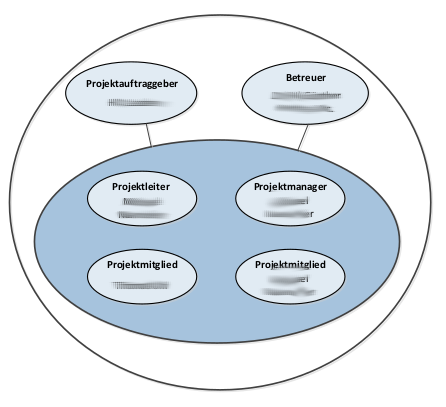
\includegraphics[width=0.5\textwidth,height=\textheight]{img/projektorganisation.png}
\caption{Projektorganisationsdiagramm}
\end{figure}

\hypertarget{vorgehen-bei-uxe4nderungen}{%
\subsubsection{Vorgehen bei
Änderungen}\label{vorgehen-bei-uxe4nderungen}}

Hier dokumentieren sie betreffend des Meilensteinplans oder der
Anwendungsfälle:

\begin{itemize}
\tightlist
\item
  Wer wird informiert,
\item
  wer muss zustimmen,
\item
  wo werden die Änderungen wie vermerkt?
\end{itemize}

Das dient in erster Linie dazu um ein einheitliches Vorgehen definiert
zu haben.

\hypertarget{meilensteine}{%
\subsection{Meilensteine}\label{meilensteine}}

Der Begriff taucht im Projektmanagement sehr häufig auf. Meilensteine
sind wichtige Punkte im Projektverlauf. Oft werden sie auch als
Prüfpunkte bezeichnet.

Generell kann ein Meilenstein ein Ereignis sein, an dem

\begin{itemize}
\tightlist
\item
  etwas abgeschlossen ist,
\item
  etwas begonnen wird oder
\item
  über die weitere Vorgehensweise entschieden wird
\end{itemize}

Meilensteine werden meist am Ende von Projektphasen definiert. Auch
innerhalb von Phasen kann es zusätzliche Meilensteine geben.

Meilensteine verlaufen nie über eine Zeitdauer. Nie. Sie sind lediglich
Entscheidungspunkte

Hier ein Beispiel wie die Meilensteine im Fall einer aussehen können

\hypertarget{projektmanagement-abgeschlossen}{%
\subsubsection{2020-09-15: Projektmanagement
abgeschlossen}\label{projektmanagement-abgeschlossen}}

\begin{itemize}
\tightlist
\item
  Projekthandbuch ist fertig
\item
  Serverinfrastruktur ist hergestellt
\item
  Bestellungen sind abgessendet
\end{itemize}

\hypertarget{genehmigung-der-da}{%
\subsubsection{2020-11-01: Genehmigung der
DA}\label{genehmigung-der-da}}

\begin{itemize}
\tightlist
\item
  Einreichen des Antrags durch die Schüler/innen
\item
  DA Dokumentation wurde ausgefüllt und unterschrieben
\end{itemize}

\hypertarget{literaturrecherche-abgeschlossen}{%
\subsubsection{2020-11-26: Literaturrecherche
abgeschlossen}\label{literaturrecherche-abgeschlossen}}

\begin{itemize}
\tightlist
\item
  Literatur zum Thema XY gesucht und in bibtex vermerkt
\item
  Aktellen Stand der Forschung erhoben
\item
  Verschriftlichung des Literaturteils begonnen
\end{itemize}

\hypertarget{prototyp-ist-funktionell}{%
\subsubsection{2020-12-17: Prototyp ist
funktionell}\label{prototyp-ist-funktionell}}

\begin{itemize}
\tightlist
\item
  DB mit Tabelle für Benutzer.
\item
  DB Kommunikation zur Anwendung (inkl. Dokumentation)
\item
  Es gibt in der Anwendung einen /Admin/ Benutzer. Dieser Benutzer kann
  weitere Benutzer in den Rollen /Lehrende/ und bzw. oder /Studierende/
  anlegen.
\end{itemize}

\hypertarget{applikation-fertiggestellt}{%
\subsubsection{2021-01-10: Applikation
fertiggestellt}\label{applikation-fertiggestellt}}

\begin{itemize}
\tightlist
\item
  Lehrende sind dazu in der Lage Tests anzulegen.
\item
  Studenten können einen ihnen zugewiesenen Test absolvieren.
\end{itemize}

\hypertarget{review-und-uxfcberarbeitung-fertig}{%
\subsubsection{2021-01-10: Review und Überarbeitung
fertig}\label{review-und-uxfcberarbeitung-fertig}}

\begin{itemize}
\tightlist
\item
  Der Quellcode ist gemeinsam mit den Projektpartnern reviewt
\item
  Quellcodedokumentation abgeschlossen (Javadoc)
\item
  Projekt baut auf eigenem Buildserver (Continous Integration)
\end{itemize}

\hypertarget{diploarbeit-fertig-verschriftlicht}{%
\subsubsection{2021-02-03: Diploarbeit fertig
verschriftlicht}\label{diploarbeit-fertig-verschriftlicht}}

\begin{itemize}
\tightlist
\item
  Stilfehler sind behoben
\item
  DA Dokumentationsblatt ist unterschrieben, eingescannt und im
  Hauptdokument enthalten
\item
  Praxisteil ist ebgeschlossen und verschriftlicht
\item
  Informationen sind im DA Portal eingegeben
\item
  Unterschriebene DA Betreuungsprotokolle sind in der DA enthalten
\item
  DA liegt dem Betreuer in ausgedruckter Form vor
\end{itemize}

\hypertarget{anwendungsfuxe4lle}{%
\subsection{Anwendungsfälle}\label{anwendungsfuxe4lle}}

Hier beschreiben Sie die Anwendungsfälle (=UseCases) Ihrer Anwendung /
Diplomarbeit. Dabei sollte die Beschreibung auf hohem Niveau (also ohne
implementierungsspezifische Details) erfolgen und typischerweise so
benannt sein, wie die Ziele aus Sicht der Akteure heißen: Mitglied
anmelden, Geld abheben, Auto zurückgeben.

Jeder Anwendungsfall wird im selben Muster beschrieben. In den folgenden
Absätzen ist zuerst eine allgemeine Beschreibung eines solchen
Anwendungsfalls zu finden und dann ein Beispiel dazu.

Damit man auch versteht wer mit welchem Anwendungsfall agiert bietet es
sich an hier eine Übersichtsgrafik zu erstellen:

\begin{figure}
\centering
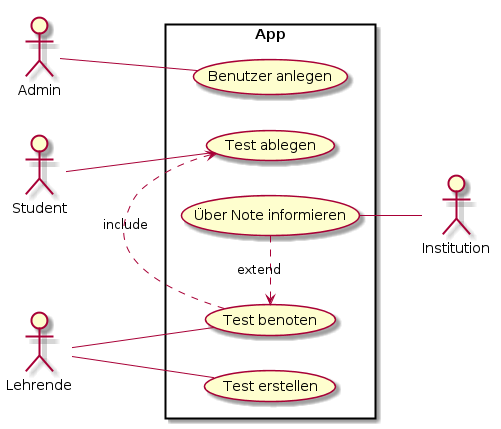
\includegraphics[width=0.6\textwidth,height=\textheight]{img/anwendungsfalldiagramm.png}
\caption{Übersicht Anwendungsfälle}
\end{figure}

\newpage

\hypertarget{anwendungsfallname}{%
\subsubsection{Anwendungsfallname}\label{anwendungsfallname}}

Anwendungsfälle haben einen eindeutigen Namen aus dem man auf den Inhalt
des Anwendungsfalls schließen kann. Wenn Sie agil arbeiten dann stellt
ein Anwendungsfall eine UserStory dar welche im Backlog liegt und im
Laufe des Projekts (in einem Sprint) abgearbeitet wird.

\hypertarget{kurzbeschreibung}{%
\paragraph{Kurzbeschreibung}\label{kurzbeschreibung}}

Hier erfolgt eine kurze Beschreibung, was im Anwendungsfall passiert.
Kurz bedeutet, dass es zwei oder drei Zeilen sind, selten mehr.

\hypertarget{trigger}{%
\paragraph{Trigger}\label{trigger}}

Der fachliche Grund bzw. die Gründe dafür, dass dieser Anwendungsfall
ausgeführt

\hypertarget{vorbedingung}{%
\paragraph{Vorbedingung}\label{vorbedingung}}

Alle Bedingungen, die erfüllt sein müssen, damit dieser Anwendungsfall
ausgeführt werden kann. Gibt es keine Vorbedingungen, so steht hier
``keine''.

\hypertarget{nachbedingung}{%
\paragraph{Nachbedingung}\label{nachbedingung}}

Der Zustand, der nach einem erfolgreichen Durchlauf des Anwendungsfalls
erwartet wird.

\hypertarget{akteure}{%
\paragraph{Akteure}\label{akteure}}

Akteure sind beteiligte Personen oder Systeme außerhalb (!) des
beschriebenen Systems. Z. B. Anwender, angemeldeter Anwender, Kunde,
System, Abrechnungsprozess.

\hypertarget{standardablauf}{%
\paragraph{Standardablauf}\label{standardablauf}}

Hier wird das typische Szenario dargestellt, das leicht zu verstehen
oder der am häufigsten vorkommende Fall ist. An seinem Ende steht die
Zielerreichung des Primärakteurs. Die Ablaufschritte werden nummeriert
und meist in strukturierter Sprache beschrieben. Ablaufpläne können
jedoch ebenfalls benutzt werden, wenn es angebracht erscheint. Mittels
der UML können diese Ablaufschritte in Aktivitätsdiagrammen oder
Anwendungsfall-orientierten Sequenzdiagrammen dargestellt werden.

\hypertarget{fehlersituationen}{%
\paragraph{Fehlersituationen}\label{fehlersituationen}}

Dies sind Szenarien, die sich außerhalb des Standardablaufs auch bei der
(versuchten) Zielerreichung des Anwendungsfalls ereignen können. Sie
werden meistens als konditionale Verzweigungen der normalen
Ablaufschritte dargestellt. An ihrem Ende steht ein Misserfolg, die
Zielerreichung des Primärakteurs oder eine Rückkehr zum Standardablauf.

\hypertarget{systemzustand-im-fehlerfall}{%
\paragraph{Systemzustand im
Fehlerfall}\label{systemzustand-im-fehlerfall}}

Der Zustand, der nach einem erfolglosen Durchlauf des Anwendungsfalls
erwartet wird.

\newpage

\hypertarget{benutzer-anlegen}{%
\subsubsection{Benutzer Anlegen}\label{benutzer-anlegen}}

\hypertarget{kurzbeschreibung-1}{%
\paragraph{Kurzbeschreibung}\label{kurzbeschreibung-1}}

Der Benutzer ``Admin'' kann auf Anfrage einen neuen Benutzer als
``Lehrende'' und bzw. oder ``Studierende'' anlegen

\hypertarget{trigger-1}{%
\paragraph{Trigger}\label{trigger-1}}

Admin legt auf Anfrage eines Benutzers einen neuen Account an

\hypertarget{vorbedingung-1}{%
\paragraph{Vorbedingung}\label{vorbedingung-1}}

Benutzer als ``Admin'' angemeldet

\hypertarget{nachbedingung-1}{%
\paragraph{Nachbedingung}\label{nachbedingung-1}}

Es existiert ein Eintrag in der DB Benutzer Tabelle für den neu
erstellten Benutzer. (Dieser kann sich anschließend in der Anwendung
anmelden)

\hypertarget{akteure-1}{%
\paragraph{Akteure}\label{akteure-1}}

\begin{itemize}
\tightlist
\item
  Admin
\end{itemize}

\hypertarget{fehlersituationen-1}{%
\paragraph{Fehlersituationen}\label{fehlersituationen-1}}

Admin bricht die Aktion ab

\hypertarget{systemzustand-im-fehlerfall-1}{%
\paragraph{Systemzustand im
Fehlerfall}\label{systemzustand-im-fehlerfall-1}}

Benutzer wird nicht angelegt und wird verworfen

\hypertarget{standardablauf-1}{%
\paragraph{Standardablauf:}\label{standardablauf-1}}

\begin{enumerate}
\def\labelenumi{\arabic{enumi}.}
\tightlist
\item
  Admin drückt Button, um einen neuen Benutzer anzulegen
\item
  Es öffnet sich ein Formular, indem die nötigen Benutzer-Informationen
  eingegeben werden (Name, Adresse, Telephonnummer, E-Mail,
  Geburtsdatum, Passwort-Hash, Rolle). Der neue Benutzer muss mindestens
  einer der Rollen ``Lehrende'' und ``Studierende'' angehören
\end{enumerate}

\hypertarget{alternativabluxe4ufe}{%
\paragraph{Alternativabläufe:}\label{alternativabluxe4ufe}}

\begin{itemize}
\tightlist
\item
  Admin drückt den Button, um die Aktion abzubrechen
\end{itemize}

\newpage

\hypertarget{dokumentation}{%
\subsection{Dokumentation}\label{dokumentation}}

Im Abschnitt Projektdokumentation können Sie mit Hilfe eines
Projektmanagementwerkzeuges Ihrer Wahl die Projektumsetzung
dokumentieren. (Also ein fortlaufender Projektfortschrittsbericht)

Normalerweise werden Sie die UserStories in mehrere SubTasks zerreissen
und dann in einem agilen verfahen (Scrum, Kanban, was auch immer ihnen
am geeignetsten erscheint) abarbeiten. Dazu können Sie natürlich eine
Softwahre Ihrer Wahl verwenden.

Am Ende sollten sie aber für jeden Projektabschnitt (Das ist die Zeit
zwischen den Meilensteinen) eine Dokumentation entstehen aus der
ersichtlich ist

\begin{itemize}
\tightlist
\item
  Berichtszeitraum
\item
  Durchgeführte Arbeiten im Berichtszeitraum sowie die Aufwände der
  einzelnen Personen
\item
  Projektstatus (Im Plan, Schwierigkeiten, Risiko)
\item
  Gesamtstatus sowie die möglicherweise notwendigen Maßnahmen für

  \begin{itemize}
  \tightlist
  \item
    Leistungsziele
  \item
    Terminziele
  \item
    Kostenziele
  \item
    Teamarbeit
  \end{itemize}
\item
  Nächste Schritte und notwendige Entscheidungen
\end{itemize}

Im folgenden Abschnitt ist ein solcher Fortschritt illustriert.

\hypertarget{projektfortschritt-01.-juni-bis-05.-august-2020}{%
\subsubsection{Projektfortschritt 01. Juni bis 05. August
2020}\label{projektfortschritt-01.-juni-bis-05.-august-2020}}

\hypertarget{gesamtstatus}{%
\paragraph{Gesamtstatus}\label{gesamtstatus}}

\begin{itemize}
\tightlist
\item
  Das Projekt befindet sich derzeit im Plan.
\item
  Es wurden alle Teile bestellt und die Hardware dimensioniert
\item
  Bei den Lieferungen hat es leichte Verspätungen gegeben
\end{itemize}

\begin{longtable}[]{@{}lll@{}}
\caption{Projektstatus am 2020-08-05}\tabularnewline
\toprule
\begin{minipage}[b]{0.30\columnwidth}\raggedright
Dimension\strut
\end{minipage} & \begin{minipage}[b]{0.27\columnwidth}\raggedright
Status\strut
\end{minipage} & \begin{minipage}[b]{0.34\columnwidth}\raggedright
Maßnahmen\strut
\end{minipage}\tabularnewline
\midrule
\endfirsthead
\toprule
\begin{minipage}[b]{0.30\columnwidth}\raggedright
Dimension\strut
\end{minipage} & \begin{minipage}[b]{0.27\columnwidth}\raggedright
Status\strut
\end{minipage} & \begin{minipage}[b]{0.34\columnwidth}\raggedright
Maßnahmen\strut
\end{minipage}\tabularnewline
\midrule
\endhead
\begin{minipage}[t]{0.30\columnwidth}\raggedright
Leistungsziele\strut
\end{minipage} & \begin{minipage}[t]{0.27\columnwidth}\raggedright
In Ordnung\strut
\end{minipage} & \begin{minipage}[t]{0.34\columnwidth}\raggedright
keine\strut
\end{minipage}\tabularnewline
\begin{minipage}[t]{0.30\columnwidth}\raggedright
Terminziele\strut
\end{minipage} & \begin{minipage}[t]{0.27\columnwidth}\raggedright
Verzug durch Lieferprobleme\strut
\end{minipage} & \begin{minipage}[t]{0.34\columnwidth}\raggedright
Bei restlichen Teilen Expresslieferung\strut
\end{minipage}\tabularnewline
\begin{minipage}[t]{0.30\columnwidth}\raggedright
Kostenziele\strut
\end{minipage} & \begin{minipage}[t]{0.27\columnwidth}\raggedright
Teile im Budget, Batterie sehr teuer\strut
\end{minipage} & \begin{minipage}[t]{0.34\columnwidth}\raggedright
Günstigere Teile bei der restlichen Hardware verwenden\strut
\end{minipage}\tabularnewline
\begin{minipage}[t]{0.30\columnwidth}\raggedright
Teamarbeit\strut
\end{minipage} & \begin{minipage}[t]{0.27\columnwidth}\raggedright
optimal\strut
\end{minipage} & \begin{minipage}[t]{0.34\columnwidth}\raggedright
keine\strut
\end{minipage}\tabularnewline
\bottomrule
\end{longtable}

\hypertarget{notwendige-entscheidungen}{%
\paragraph{Notwendige Entscheidungen}\label{notwendige-entscheidungen}}

\begin{itemize}
\tightlist
\item
  Die Zusammenbauphase muss etwas verschoben werden und startet nun um
  14 Tage später. Das hat keinen Einfluss auf den Endtermin.
\end{itemize}

\hypertarget{nuxe4chste-schritte}{%
\paragraph{Nächste Schritte}\label{nuxe4chste-schritte}}

\begin{itemize}
\tightlist
\item
  Abklären ob die Expressbestellungen im Budget sind
\item
  Start dder Implementierungsphase
\end{itemize}

: Projektstatus Stand 05. August 2020

\newpage

\hypertarget{projektabschlussbericht}{%
\subsection{Projektabschlussbericht}\label{projektabschlussbericht}}

\hypertarget{erfolgsmessung}{%
\subsubsection{Erfolgsmessung}\label{erfolgsmessung}}

\hypertarget{erreichung-leistungs-qualituxe4tsziele}{%
\paragraph{Erreichung
Leistungs-/Qualitätsziele}\label{erreichung-leistungs-qualituxe4tsziele}}

Hier beschreibe sie ob Sie das ursprünglich vereinbarte Ziel erreicht
haben oder nicht. Falls es zu irgendwelchen Abweichungen gekommen ist
dann beschreiben Sie warum das so war und was Sie dagegen unternommen
haben.

\hypertarget{erreichung-terminziele}{%
\paragraph{Erreichung Terminziele}\label{erreichung-terminziele}}

Hier dokumentieren Sie ob Sie Ihre gesteckten Termine für die
Meilensteine einhalten konnten. Falls es zu verzügen gekommen ist
argumentieren sie hier warum das so war.

\hypertarget{erreichung-kosten-aufwandsziele}{%
\paragraph{Erreichung
Kosten-/Aufwandsziele}\label{erreichung-kosten-aufwandsziele}}

Hier dokumentieren Sie ob Sie Ihr eingangs geplantes Budget einhalten
konnten oder nicht. Wenn nicht geben Sie hier bitte eine Begümdung dafür
an.

\hypertarget{refelxion-lessons-learned}{%
\subsubsection{Refelxion / Lessons
Learned}\label{refelxion-lessons-learned}}

\hypertarget{teamarbeit}{%
\paragraph{Teamarbeit}\label{teamarbeit}}

Hier dokumentieren sie Ihre Erkenntnisse bezüglich der Teamarbeit in
Ihrem Projekt. Was ist gut gelaufen und was schlecht ?

\hypertarget{projektmanagement}{%
\paragraph{Projektmanagement}\label{projektmanagement}}

Hier dokumentieren sie Ihre Erkenntnisse bezüglich des
Projektmanagements.

\hypertarget{sonstige-lernerfahrungen}{%
\paragraph{Sonstige Lernerfahrungen}\label{sonstige-lernerfahrungen}}

Hier dokuentieren was sie im Bezug auf das Projekt sonst noch so gelernt
haben

\hypertarget{nachhaltigkeitsanalyse}{%
\subsubsection{Nachhaltigkeitsanalyse}\label{nachhaltigkeitsanalyse}}

In diesem verpflichtenden Abschnitt dokumentieren Sie wie sich Ihre
Arbeit im Bezug auf die \href{https://sdgs.un.org/goals}{17 Sustainable
Development Goals} eingliedert und auswirkt. Im Speziellen erörtern Sie
welche Punkte davon Betroffen sind und wo Ihre Arbeit hier einen
positiven (oder auch negativen) Beitrag leistet. \singlespacing

\translatelet\lof{lstoffigures}
\section{ \lof }
\listoffigures

\translatelet\lot{lstoftables}
\section{ \lot }
\listoftables

\translatelet\lol{lstoflistings}
\section{ \lol }
\lstlistoflistings

\translatelet\lor{lstofreferences}
\section{ \lor }

\hypertarget{refs}{}
\leavevmode\hypertarget{ref-hattie_lernen_2013}{}%
1 . \textbf{Hattie John, Beywl Wolfgang und Zierer Klaus} (2013)
\emph{Lernen sichtbar machen}, Baltmannsweiler, Schneider-Verl.
Hohengehren., ISBN:
\href{https://worldcat.org/isbn/978-3-8340-1190-9}{978-3-8340-1190-9},
OCLC: 844027245

\leavevmode\hypertarget{ref-heise}{}%
2 . \textbf{Bez Roberto} (2014) „CSS-Präprozessoren im Vergleich``.
{[}online{]} (Zugegriffen 14 August 2016)
\url{http://www.heise.de/developer/artikel/CSS-Praeprozessoren-im-Vergleich-2288284.html}

\leavevmode\hypertarget{ref-t3n}{}%
3 . \textbf{Janschitz Mario} (2015) „Sass vs. Less: So findest du den
richtigen Präprozessor für dich``. {[}online{]} (Zugegriffen 17 Juli
2016) \url{http://t3n.de/news/sass-vs-less-636820/}

\leavevmode\hypertarget{ref-leeb_einfuhrung_2016}{}%
4 . \textbf{Leeb Christine, Leitner Rita, Pichler Verena, Huber-Gries
Carina, u.~a.} (2016) „Einführung und Optimierung eines
praxisorientierten Problem-based-Learning-Moduls im
Life-Science-Bereich``. \emph{Zeitschrift für Hochschulentwicklung}.
{[}online{]} (Zugegriffen 15 August 2016)
\url{http://www.zfhe.at/index.php/zfhe/article/view/897}

\leavevmode\hypertarget{ref-Zatko15}{}%
5 . \textbf{Zatko Peiter, Poupyrev Ivan, El Guerrab Rachid und Dugan
Regina} (2015) „Google I/O 2015. A little badass. Beautiful. Tech and
human. Work and love. ATAP``. {[}online{]} (Zugegriffen 23 Dezember
2020) \url{https://www.youtube.com/watch?v=mpbWQbkl8_g}

\leavevmode\hypertarget{ref-gpt-pandoc}{}%
6 . \textbf{ChatGPT 4.0} (2024) „Was ist Pandoc ?`` {[}online{]}
(Zugegriffen 29 Februar 2023)
\url{https://chat.openai.com/c/ef535195-0e39-4d5c-9c85-cdb7ec18ad03}

\leavevmode\hypertarget{ref-gpt-atomaufbau}{}%
7 . \textbf{ChatGPT} (2024) „Aufbau eines Atoms``. {[}online{]}
(Zugegriffen 29 Februar 2023)
\url{https://chat.openai.com/c/0484c9c2-fe7f-4922-af0b-76c3ca15fb58}

\renewcommand{\authormark}{}% Ab hier keine Authorangaben mehr
\cleardoublepage{}
%%%%%%%%%%%%%%%%%%%%%%%%%%%%%%%%%%%%%%%%%%%%%%%%%%%%%%%%%%%%%%%%%%%%%%%%%%%%%%%%
%  VERZEICHNISSE
%%%%%%%%%%%%%%%%%%%%%%%%%%%%%%%%%%%%%%%%%%%%%%%%%%%%%%%%%%%%%%%%%%%%%%%%%%%%%%%%
% ... werden über die Datei 'verzeichnisse.md' von Pandoc nach Latex 
% kompiliert und am Ende der Arbeit angehängt

% Normalerweise kommen die Verzeichnisse in dieser Reihenfolge:
% 1.) Abbildungsverzeichnis
% 2.) Tabellenverzeichnis
% 3.) Literaturverzeichnis 


%%%%%%%%%%%%%%%%%%%%%%%%%%%%%%%%%%%%%%%%%%%%%%%%%%%%%%%%%%%%%%%%%%%%%%%%%%%%%%%%
%  KI Quellen
%%%%%%%%%%%%%%%%%%%%%%%%%%%%%%%%%%%%%%%%%%%%%%%%%%%%%%%%%%%%%%%%%%%%%%%%%%%%%%%%
% ... besteht aus PDF Files die in der metadata.yaml Datei deklariert werden
% und hier dann eingebunden werden. Normalerweise sind das folgende Dateien

\translatelet\app{aisources}
\section{\app}

\translate{attachments}
\begin{itemize}

\item \textbf{ChatGPT4: Erklärung Pandoc}\\  Datei: \texttt{gpt-pandoc.pdf}
\item \textbf{ChatGPT3.5: Aufbau eines Atoms}\\  Datei: \texttt{gpt-atom.pdf}
\end{itemize}


\stepcounter{subsection}
\phantomsection
\addcontentsline{toc}{subsection}{\protect\numberline{\thesubsection}ChatGPT4: Erklärung Pandoc}

\includepdf[
    clip=0mm 0mm 0mm 0mm,
    pages=-,
    frame,
    scale=.73,
    pagecommand={\begin{center}\translate{attachment}: Erklärung Pandoc\\\begin{tiny}gpt-pandoc.pdf\end{tiny}\end{center}}
 ]{pdfs/gpt-pandoc.pdf}
%\includepdf[pages=-]{source/pdfs/}
\stepcounter{subsection}
\phantomsection
\addcontentsline{toc}{subsection}{\protect\numberline{\thesubsection}ChatGPT3.5: Aufbau eines Atoms}
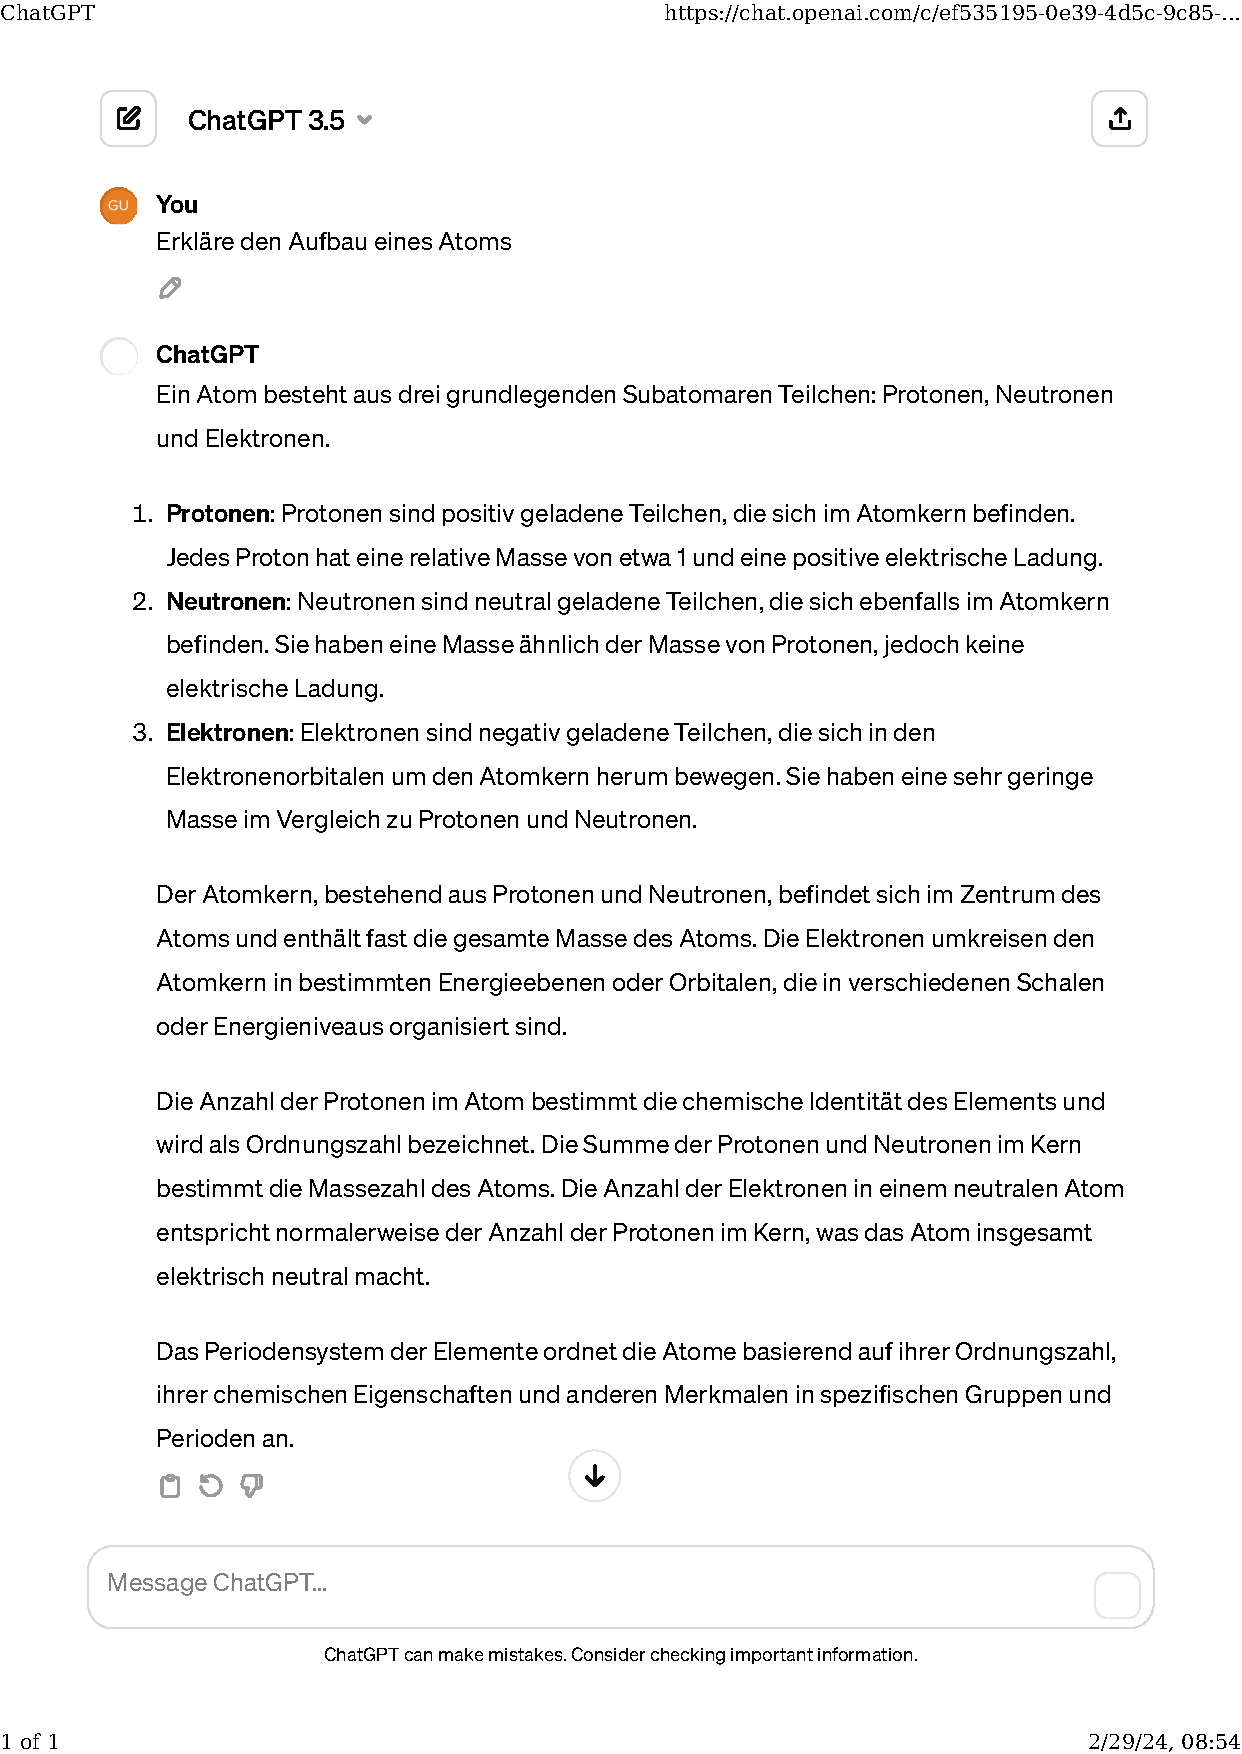
\includepdf[
    clip=0mm 0mm 0mm 0mm,
    pages=-,
    frame,
    scale=.73,
    pagecommand={\begin{center}\translate{attachment}: Aufbau eines Atoms\\\begin{tiny}gpt-atom.pdf\end{tiny}\end{center}}
 ]{pdfs/gpt-atom.pdf}
%\includepdf[pages=-]{source/pdfs/}

%%%%%%%%%%%%%%%%%%%%%%%%%%%%%%%%%%%%%%%%%%%%%%%%%%%%%%%%%%%%%%%%%%%%%%%%%%%%%%%%
%  APPENDIX
%%%%%%%%%%%%%%%%%%%%%%%%%%%%%%%%%%%%%%%%%%%%%%%%%%%%%%%%%%%%%%%%%%%%%%%%%%%%%%%%
% ... besteht aus PDF Files die in der metadata.yaml Datei deklariert werden
% und hier dann eingebunden werden. Normalerweise sind das folgende Dateien

% BEGLEITPROTOKOLLE
% PROJEKTHANDBUCH
% TECHNISCHE DOKUMENTATION
% ERKLAERUNG ZUR DA

\translatelet\app{appendix}
\section{\app}

\translate{attachments}
\begin{itemize}

\item \textbf{Technische Dokumentation}\\ \translate{pages} 53-73 \translate{of}  Datei: \texttt{pandoc-manual.pdf}
\item \textbf{Betreuungsprotokolle}\\  Datei: \texttt{betreuungsprotokolle.pdf}
\item \textbf{Diplomatbeitsvereinbarung Englisch}\\  Datei: \texttt{HTL-DA-Doku-EN.pdf}
\item \textbf{Diplomatbeitsvereinbarung Deutsch}\\  Datei: \texttt{HTL-DA-Doku-DE.pdf}
\end{itemize}


%\subsection{Technische Dokumentation}
\stepcounter{subsection}
\phantomsection
\addcontentsline{toc}{subsection}{\protect\numberline{\thesubsection}Technische Dokumentation}

\includepdf[
    clip=0mm 0mm 0mm 0mm,
    pages=53-73,
    frame,
    scale=.73,
    pagecommand={\begin{center}\translate{attachment}: Technische Dokumentation\\\begin{tiny}pandoc-manual.pdf\end{tiny}\end{center}}
 ]{pdfs/pandoc-manual.pdf}
%
\includepdf[pages=53-73]{source/pdfs/pandoc-manual.pdf}
%\subsection{Betreuungsprotokolle}
\stepcounter{subsection}
\phantomsection
\addcontentsline{toc}{subsection}{\protect\numberline{\thesubsection}Betreuungsprotokolle}

\includepdf[
    clip=0mm 0mm 0mm 0mm,
    pages=-,
    frame,
    scale=.73,
    pagecommand={\begin{center}\translate{attachment}: Betreuungsprotokolle\\\begin{tiny}betreuungsprotokolle.pdf\end{tiny}\end{center}}
 ]{pdfs/betreuungsprotokolle.pdf}
%
\includepdf[pages=-]{source/pdfs/betreuungsprotokolle.pdf}
%\subsection{Diplomatbeitsvereinbarung Englisch}
\stepcounter{subsection}
\phantomsection
\addcontentsline{toc}{subsection}{\protect\numberline{\thesubsection}Diplomatbeitsvereinbarung Englisch}
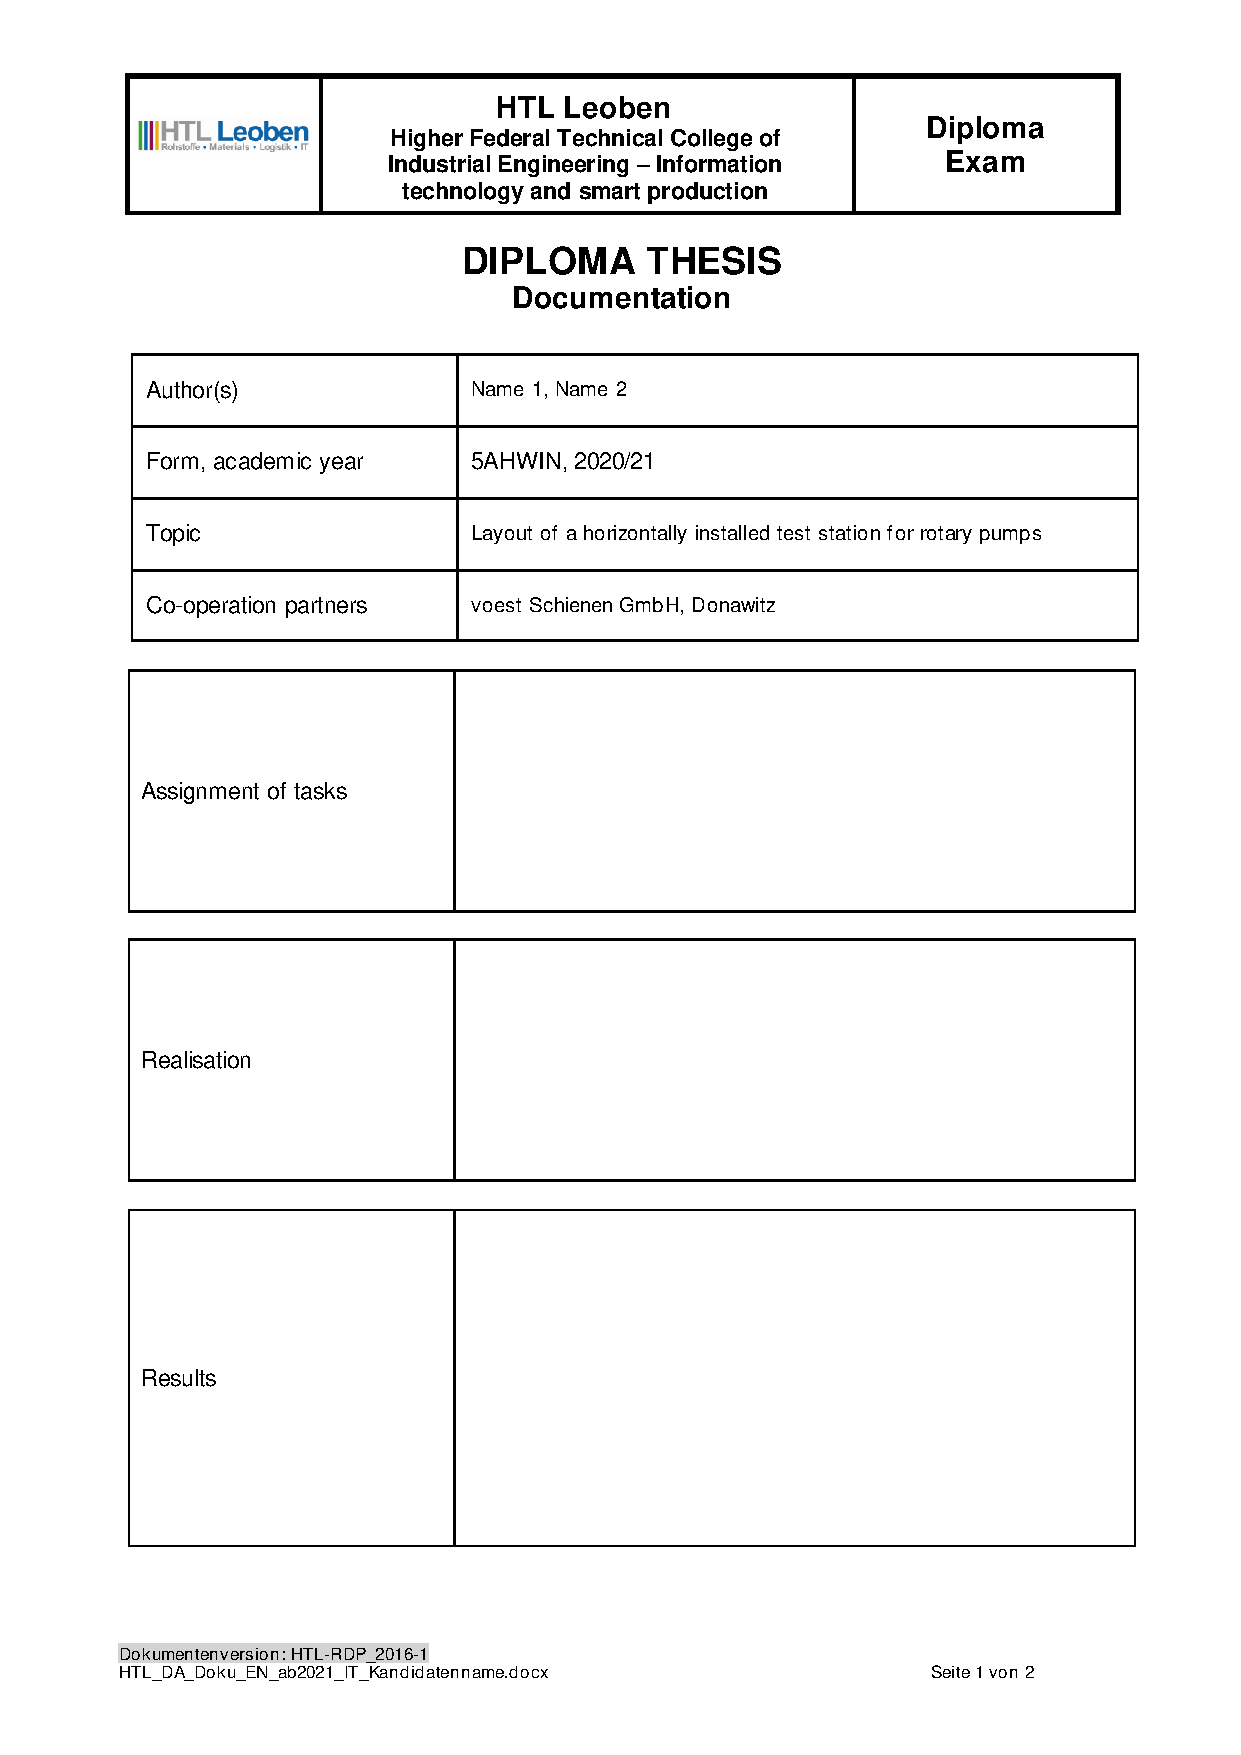
\includepdf[
    clip=0mm 0mm 0mm 0mm,
    pages=-,
    frame,
    scale=.73,
    pagecommand={\begin{center}\translate{attachment}: Diplomatbeitsvereinbarung Englisch\\\begin{tiny}HTL-DA-Doku-EN.pdf\end{tiny}\end{center}}
 ]{pdfs/HTL-DA-Doku-EN.pdf}
%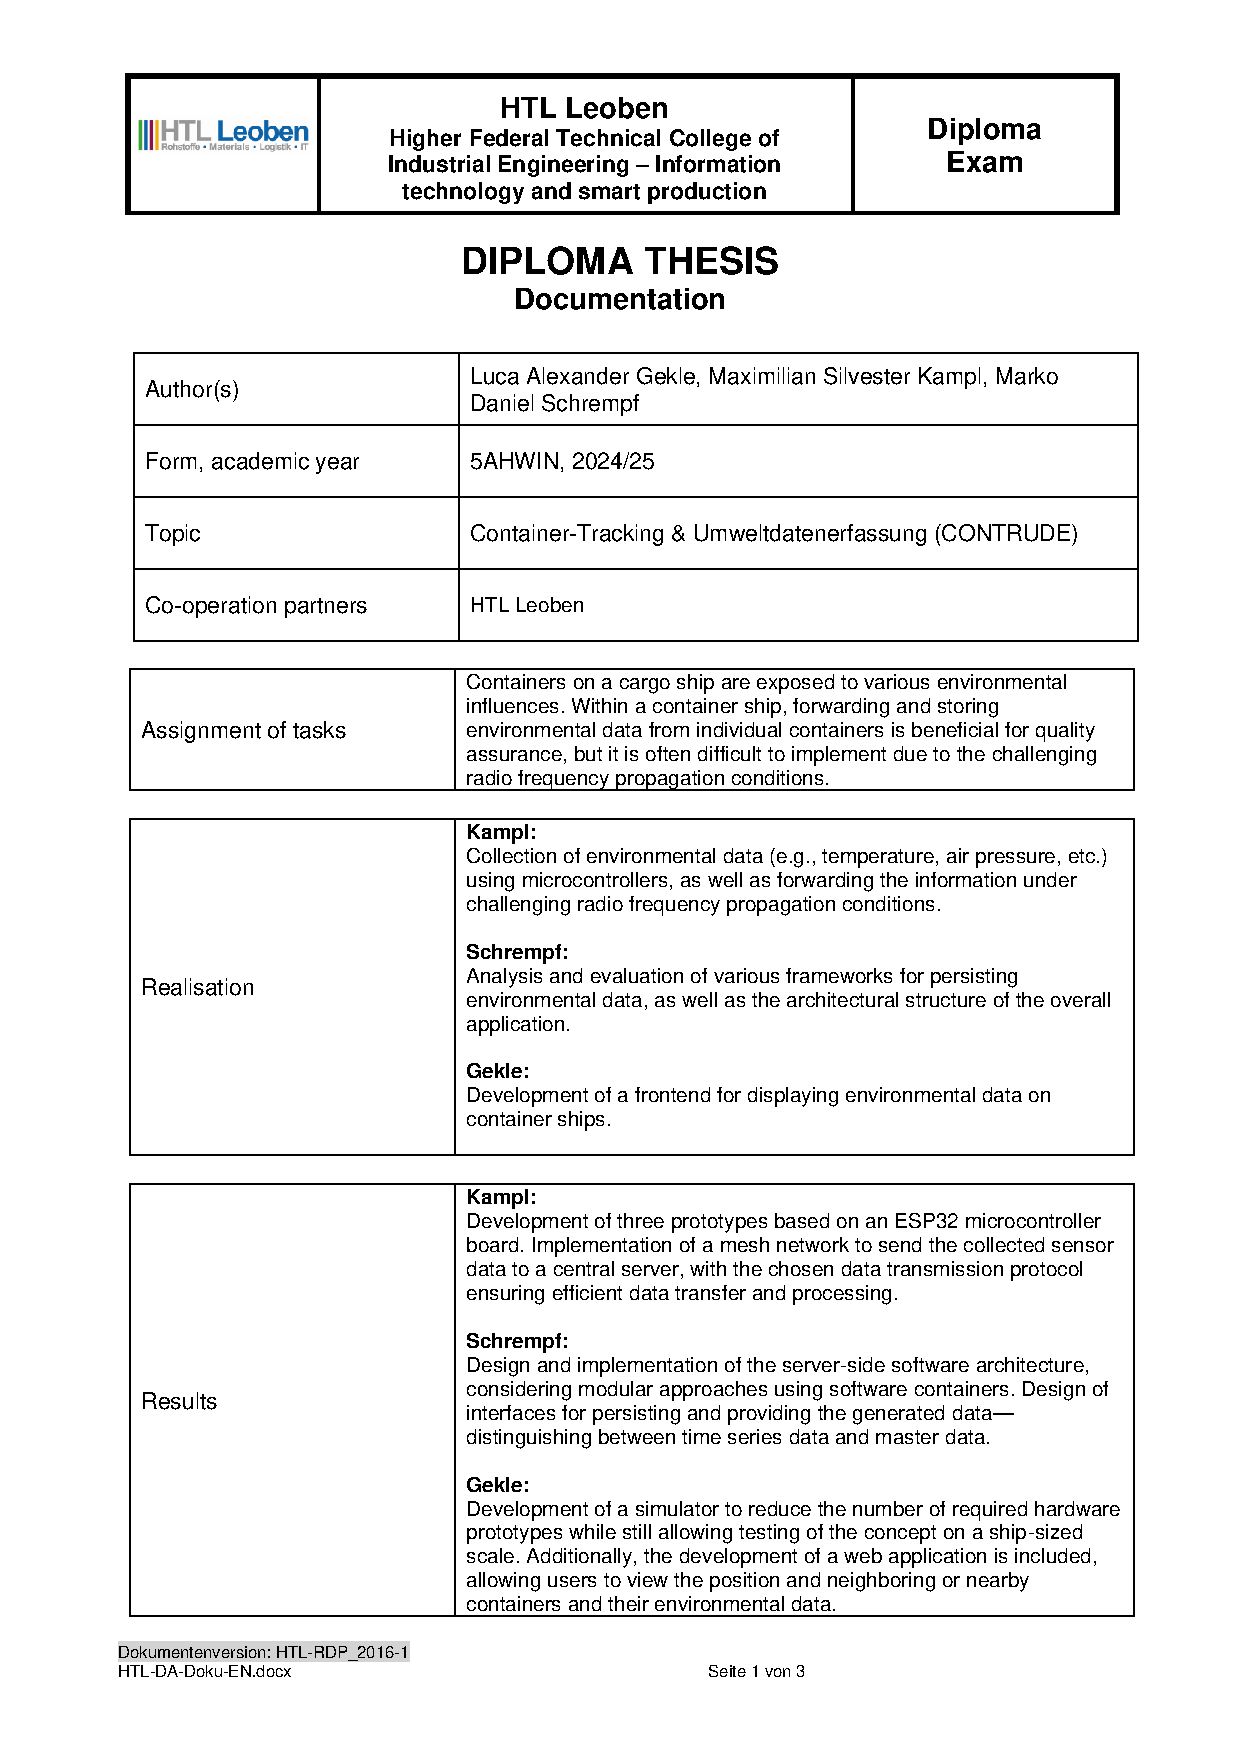
\includepdf[pages=-]{source/pdfs/HTL-DA-Doku-EN.pdf}
%\subsection{Diplomatbeitsvereinbarung Deutsch}
\stepcounter{subsection}
\phantomsection
\addcontentsline{toc}{subsection}{\protect\numberline{\thesubsection}Diplomatbeitsvereinbarung Deutsch}
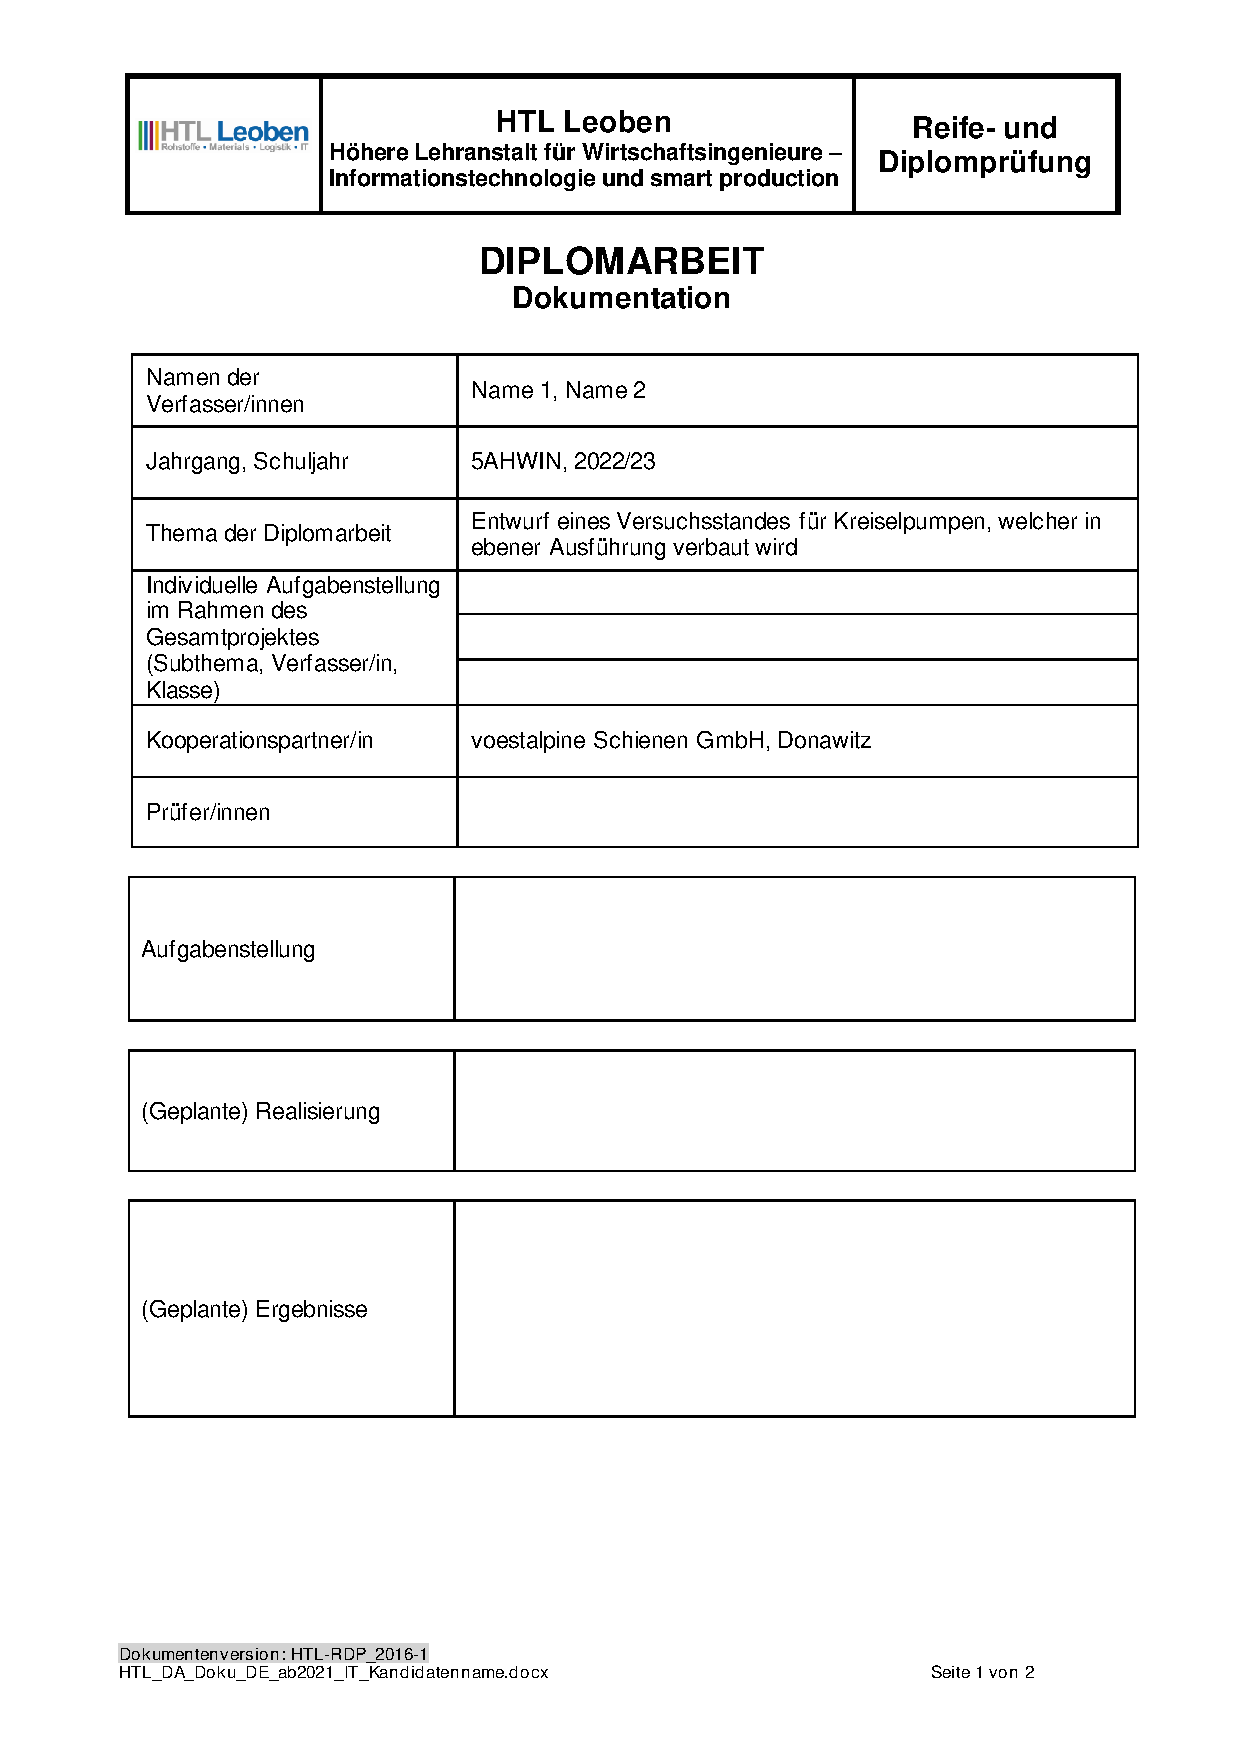
\includepdf[
    clip=0mm 0mm 0mm 0mm,
    pages=-,
    frame,
    scale=.73,
    pagecommand={\begin{center}\translate{attachment}: Diplomatbeitsvereinbarung Deutsch\\\begin{tiny}HTL-DA-Doku-DE.pdf\end{tiny}\end{center}}
 ]{pdfs/HTL-DA-Doku-DE.pdf}
%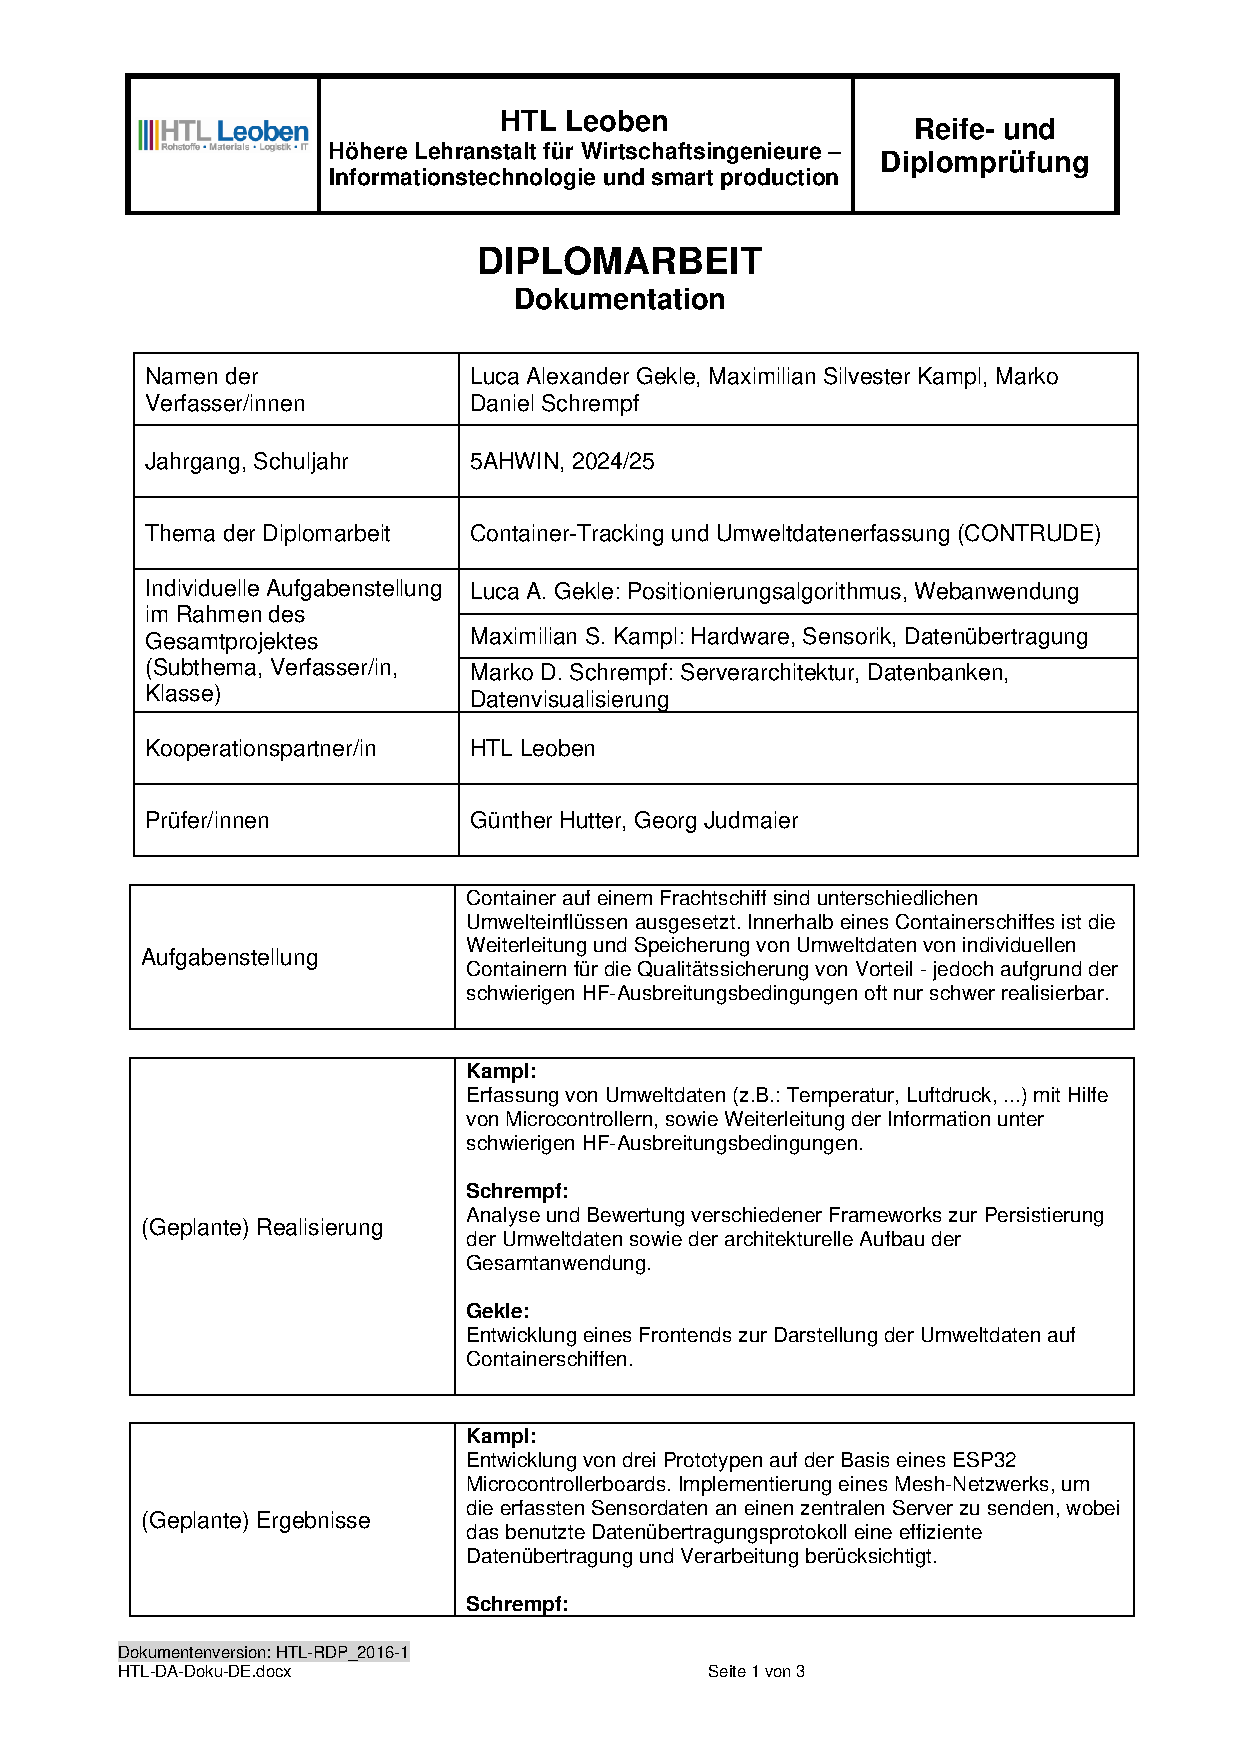
\includepdf[pages=-]{source/pdfs/HTL-DA-Doku-DE.pdf}

\end{document}

